\documentclass{report}
%%%%%%%%%%%%%% preamble.tex %%%%%%%%%%%%%%
\usepackage[T1]{fontenc}
\usepackage{etoolbox}
% Page Setup
\usepackage[letterpaper, tmargin=2cm, rmargin=0.5in, lmargin=0.5in, bmargin=80pt, footskip=.2in]{geometry}
\usepackage{adjustbox}
\usepackage{graphicx}
\usepackage{tikz}
\usepackage{mathrsfs}
\usepackage{mdframed}

% Create a new toggle
\newtoggle{firstsection}

% Redefine the \chapter command to reset the toggle for each new chapter
\let\oldchapter\chapter
\renewcommand{\chapter}{\toggletrue{firstsection}\oldchapter}

% Redefine the \section command to check the toggle
\let\oldsection\section
\renewcommand{\section}{
    \iftoggle{firstsection}
    {\togglefalse{firstsection}} % If it's the first section, just switch off the toggle for next sections
    {\clearpage} % If it's not the first section, start a new page
    \oldsection
}

% Abstract Design

\usepackage{lipsum}

\renewenvironment{abstract}
 {% Start of environment
  \quotation
  \small
  \noindent
  \rule{\linewidth}{.5pt} % Draw the rule to match the linewidth
  \par\smallskip
  {\centering\bfseries\abstractname\par}\medskip
 }
 {% End of environment
  \par\noindent
  \rule{\linewidth}{.5pt} % Ensure the closing rule also matches
  \endquotation
 }

% Mathematics
\usepackage{amsmath,amsfonts,amsthm,amssymb,mathtools}
\usepackage{xfrac}
\usepackage[makeroom]{cancel}
\usepackage{enumitem}
\usepackage{nameref}
\usepackage{multicol,array}
\usepackage{tikz-cd}
\usepackage{array}
\usepackage{multirow}% http://ctan.org/pkg/multirow
\usepackage{graphicx}

% Colors
\usepackage[dvipsnames]{xcolor}
\definecolor{myg}{RGB}{56, 140, 70}
\definecolor{myb}{RGB}{45, 111, 177}
\definecolor{myr}{RGB}{199, 68, 64}
% Define more colors here...
\definecolor{olive}{HTML}{6B8E23}
\definecolor{orange}{HTML}{CC5500}
\definecolor{brown}{HTML}{8B4513}
% Hyperlinks
\usepackage{bookmark}
\usepackage[colorlinks=true,linkcolor=blue,urlcolor=blue,citecolor=blue,anchorcolor=blue]{hyperref}
\usepackage{xcolor}
\hypersetup{
    colorlinks,
    linkcolor={red!50!black},
    citecolor={blue!50!black},
    urlcolor={blue!80!black}
}

% Text-related
\usepackage{blindtext}
\usepackage{fontsize}
\changefontsize[14]{14}
\setlength{\parindent}{0pt}
\linespread{1.2}

% Theorems and Definitions
\usepackage{amsthm}
\renewcommand\qedsymbol{$\blacksquare$}

% Define a new theorem style
\newtheoremstyle{mytheoremstyle}% name
  {}% Space above
  {}% Space below
  {}% Body font
  {}% Indent amount
  {\bfseries}% Theorem head font
  {.}% Punctuation after theorem head
  {.5em}% Space after theorem head
  {}% Theorem head spec (can be left empty, meaning ‘normal’)

% Apply the new theorem style to theorem-like environments
\theoremstyle{mytheoremstyle}

\newtheorem{theorem}{Theorem}[section]  
\newtheorem{definition}[theorem]{Definition} 
\newtheorem{lemma}[theorem]{Lemma}  
\newtheorem{corollary}[theorem]{Corollary}
\newtheorem{axiom}[theorem]{Axiom}
\newtheorem{example}[theorem]{Example}
\newtheorem{equiv_def}[theorem]{Equivalent Definition}

% tcolorbox Setup
\usepackage[most,many,breakable]{tcolorbox}
\tcbuselibrary{theorems}

% Define custom tcolorbox environments here...

%================================
% EXAMPLE BOX
%================================
% After you have defined the style and other theorem environments
\definecolor{myexamplebg}{RGB}{245, 245, 245} % Very light grey for background
\definecolor{myexamplefr}{RGB}{120, 120, 120} % Medium grey for frame
\definecolor{myexampleti}{RGB}{60, 60, 60}    % Darker grey for title

\newtcbtheorem[]{Example}{Example}{
    colback=myexamplebg,
    breakable,
    colframe=myexamplefr,
    coltitle=myexampleti,
    boxrule=1pt,
    sharp corners,
    detach title,
    before upper=\tcbtitle\par\vspace{-20pt}, % Reduced the space after the title
    fonttitle=\bfseries,
    description font=\mdseries,
    separator sign none,
    description delimiters={}{}, % No delimiters around the title
}{ex}
%================================
% Solution BOX
%================================
\makeatletter
\newtcolorbox{solution}{enhanced,
	breakable,
	colback=white,
	colframe=myg!80!black,
	attach boxed title to top left={yshift*=-\tcboxedtitleheight},
	title=Solution,
	boxed title size=title,
	boxed title style={%
			sharp corners,
			rounded corners=northwest,
			colback=tcbcolframe,
			boxrule=0pt,
		},
	underlay boxed title={%
			\path[fill=tcbcolframe] (title.south west)--(title.south east)
			to[out=0, in=180] ([xshift=5mm]title.east)--
			(title.center-|frame.east)
			[rounded corners=\kvtcb@arc] |-
			(frame.north) -| cycle;
		},
}
\makeatother

% %================================
% % Question BOX
% %================================
\makeatletter
\newtcbtheorem{question}{Question}{enhanced,
	breakable,
	colback=white,
	colframe=myb!80!black,
	attach boxed title to top left={yshift*=-\tcboxedtitleheight},
	fonttitle=\bfseries,
	title={#2},
	boxed title size=title,
	boxed title style={%
			sharp corners,
			rounded corners=northwest,
			colback=tcbcolframe,
			boxrule=0pt,
		},
	underlay boxed title={%
			\path[fill=tcbcolframe] (title.south west)--(title.south east)
			to[out=0, in=180] ([xshift=5mm]title.east)--
			(title.center-|frame.east)
			[rounded corners=\kvtcb@arc] |-
			(frame.north) -| cycle;
		},
	#1
}{question}
\makeatother

%%%%%%%%%%%%%%%%%%%%%%%%%%%%%%%%%%%%%%%%%%%
% TABLE OF CONTENTS
%%%%%%%%%%%%%%%%%%%%%%%%%%%%%%%%%%%%%%%%%%%


\usepackage{tikz}
\definecolor{doc}{RGB}{0,60,110}
\usepackage{titletoc}
\contentsmargin{0cm}
\titlecontents{chapter}[14pc]
{\addvspace{30pt}%
	\begin{tikzpicture}[remember picture, overlay]%
		\draw[fill=doc!60,draw=doc!60] (-7,-.1) rectangle (-0.9,.5);%
		\pgftext[left,x=-5.5cm,y=0.2cm]{\color{white}\Large\sc\bfseries Chapter\ \thecontentslabel};%
	\end{tikzpicture}\color{doc!60}\large\sc\bfseries}%
{}
{}
{\;\titlerule\;\large\sc\bfseries Page \thecontentspage
	\begin{tikzpicture}[remember picture, overlay]
		\draw[fill=doc!60,draw=doc!60] (2pt,0) rectangle (4,0.1pt);
	\end{tikzpicture}}%
\titlecontents{section}[3.7pc]
{\addvspace{2pt}}
{\contentslabel[\thecontentslabel]{3pc}}
{}
{\hfill\small \thecontentspage}
[]
\titlecontents*{subsection}[3.7pc]
{\addvspace{-1pt}\small}
{}
{}
{\ --- \small\thecontentspage}
[ \textbullet\ ][]

\makeatletter
\renewcommand{\tableofcontents}{
	\chapter*{%
	  \vspace*{-20\p@}%
	  \begin{tikzpicture}[remember picture, overlay]%
		  \pgftext[right,x=15cm,y=0.2cm]{\color{doc!60}\Huge\sc\bfseries \contentsname};%
		  \draw[fill=doc!60,draw=doc!60] (13,-.75) rectangle (20,1);%
		  \clip (13,-.75) rectangle (20,1);
		  \pgftext[right,x=15cm,y=0.2cm]{\color{white}\Huge\sc\bfseries \contentsname};%
	  \end{tikzpicture}}%
	\@starttoc{toc}}
\makeatother

\newcommand{\liff}{\llap{$\iff$}}
\newcommand{\rap}[1]{\rrap{\text{ (#1)}}}
\newcommand{\red}[1]{\textcolor{red}{#1}}
\newcommand{\blue}[1]{\textcolor{blue}{#1}}
\newcommand{\vi}[1]{\textcolor{violet}{#1}}
\newcommand{\olive}[1]{\textcolor{olive}{#1}}
\newcommand{\teal}[1]{\textcolor{teal}{#1}}
\newcommand{\brown}[1]{\textcolor{brown}{#1}}
\newcommand{\orange}[1]{\textcolor{orange}{#1}}
\newcommand{\tCaC}{\text{ \CaC }}
\newcommand{\CaC}{\red{CaC} }
\newcommand{\As}[1]{Assume \red{#1}}
\newcommand{\vdone}{\vi{\text{ (done) }}}
\newcommand{\bdone}{\blue{\text{ (done) }}}
\newcommand{\tdone}{\teal{\text{ (done) }}}
\newcommand{\odone}{\olive{\text{ (done) }}}
\newcommand{\bodone}{\brown{\text{ (done) }}}
\newcommand{\ordone}{\orange{\text{ (done) }}}
\newcommand{\ld}{\lambda}
\newcommand{\vecta}[1]{\textbf{#1}}
\newcommand{\set}[1]{\left\{ #1 \right\}}
\newcommand{\bset}[1]{\Big\{ #1 \Big\}}
\newcommand{\inR}{\in\R}
\newcommand{\inn}{\in\N}
\newcommand{\inz}{\in\Z}
\newcommand{\inr}{\in\R}
\newcommand{\inc}{\in\C}
\newcommand{\inq}{\in\Q}
\newcommand{\norm}[1]{\| #1 \|}
\newcommand{\bnorm}[1]{\Big\| #1 \Big\|}
\newcommand{\gen}[1]{\langle #1 \rangle}
\newcommand{\abso}[1]{\left|#1\right|}
\newcommand{\myref}[2]{\hyperref[#2]{#1\ \ref*{#2}}}
\newcommand{\customref}[2]{\hyperref[#1]{#2}}
\newcommand{\power}[1]{\mathcal{P}(#1)}
\newcommand{\dcup}{\mathbin{\dot{\cup}}}
\newcommand{\diam}[1]{\text{diam}\, #1}
\newcommand{\at}{\Big|}
\newcommand{\quotient}{\diagup}
\let\originalphi\phi % Store the original \phi in \originalphi
\renewcommand{\phi}{\varphi} % Redefine \phi to \varphi
\newcommand{\pfi}{\originalphi} % Define \pfi to display the original \phi
\newcommand{\diota}{\dot{\iota}}
\newcommand{\Log}{\operatorname{Log}}
\newcommand{\id}{\text{\textbf{id}}}
\usepackage{amsmath}

\makeatletter
\NewDocumentCommand{\extp}{e{^}}{%
  \mathop{\mathpalette\extp@{#1}}\nolimits
}
\NewDocumentCommand{\extp@}{mm}{%
  \bigwedge\nolimits\IfValueT{#2}{^{\extp@@{#1}#2}}%
  \IfValueT{#1}{\kern-2\scriptspace\nonscript\kern2\scriptspace}%
}
\newcommand{\extp@@}[1]{%
  \mkern
    \ifx#1\displaystyle-1.8\else
    \ifx#1\textstyle-1\else
    \ifx#1\scriptstyle-1\else
    -0.5\fi\fi\fi
  \thinmuskip
}
\makeatletter
\usepackage{pifont}
\makeatletter
\newcommand\Pimathsymbol[3][\mathord]{%
  #1{\@Pimathsymbol{#2}{#3}}}
\def\@Pimathsymbol#1#2{\mathchoice
  {\@Pim@thsymbol{#1}{#2}\tf@size}
  {\@Pim@thsymbol{#1}{#2}\tf@size}
  {\@Pim@thsymbol{#1}{#2}\sf@size}
  {\@Pim@thsymbol{#1}{#2}\ssf@size}}
\def\@Pim@thsymbol#1#2#3{%
  \mbox{\fontsize{#3}{#3}\Pisymbol{#1}{#2}}}
\makeatother
% the next two lines are needed to avoid LaTeX substituting upright from another font
\input{utxmia.fd}
\DeclareFontShape{U}{txmia}{m}{n}{<->ssub * txmia/m/it}{}
% you may also want
\DeclareFontShape{U}{txmia}{bx}{n}{<->ssub * txmia/bx/it}{}
% just in case
%\DeclareFontShape{U}{txmia}{l}{n}{<->ssub * txmia/l/it}{}
%\DeclareFontShape{U}{txmia}{b}{n}{<->ssub * txmia/b/it}{}
% plus info from Alan Munn at https://tex.stackexchange.com/questions/290165/how-do-i-get-a-nicer-lambda?noredirect=1#comment702120_290165
\newcommand{\pilambdaup}{\Pimathsymbol[\mathord]{txmia}{21}}
\renewcommand{\lambda}{\pilambdaup}
\renewcommand{\tilde}{\widetilde}
\DeclareMathOperator*{\esssup}{ess\,sup}
\newcommand{\bluecheck}{}%
\DeclareRobustCommand{\bluecheck}{%
  \tikz\fill[scale=0.4, color=blue]
  (0,.35) -- (.25,0) -- (1,.7) -- (.25,.15) -- cycle;%
}


\usepackage{tikz}
\newcommand*{\DashedArrow}[1][]{\mathbin{\tikz [baseline=-0.25ex,-latex, dashed,#1] \draw [#1] (0pt,0.5ex) -- (1.3em,0.5ex);}}

\newcommand{\C}{\mathbb{C}}	
\newcommand{\F}{\mathbb{F}}
\newcommand{\N}{\mathbb{N}}
\newcommand{\Q}{\mathbb{Q}}
\newcommand{\R}{\mathbb{R}}
\newcommand{\Z}{\mathbb{Z}}



\title{\Huge{NCKU 112.2}\\
Geometry 1}
\author{\huge{Eric Liu}}
\date{}
\begin{document}
\maketitle
\newpage% or \cleardoublepage
% \pdfbookmark[<level>]{<title>}{<dest>}
\pdfbookmark[section]{\contentsname}{toc}
\tableofcontents
\pagebreak
\chapter{Curve}
\section{Frenet Trihedron}
\begin{mdframed}
In this section, we will use $I$ to denote an \textbf{bounded open interval}. By a \textbf{curve} in $\R^n$, we mean a function form an open interval $I$ to $\R^n$.  We say a curve is \textbf{differentiable} if it is infinitely differentiable (smooth). That is, $\gamma ^{(n)}(t)$ exists and are continuous for all $n\inn$ and $t \in I$.\\

We say a differentiable curve $\gamma  :I\rightarrow \R^n$ is \textbf{regular} if $\gamma '(t)\neq 0$ for all $t  \in I$. We say a differentiable curve $\gamma :I\rightarrow \R^n$ is a \textbf{parametrized by arc-length} if $\abso{\gamma '(t)}=1$ for all $t \in I$. 
\end{mdframed}
\begin{mdframed}
For a regular curve $\gamma $, we say $\gamma '(t)$ is the \textbf{tangent vector} of $\gamma $ at $t$, and we define the \textbf{unit tangent vector} $T$ by    
\begin{align*}
T(t)\triangleq \frac{\gamma '(t)}{\abso{\gamma '(t)}}
\end{align*}
We say $\gamma ''(t)$ is the \textbf{oriented curvature} (normal vector) of $\gamma $ at $t$, and we define the  \textbf{unit normal vector} $N$ by 
 \begin{align*}
N(t)\triangleq \frac{T'(t)}{\abso{T'(t)}}=\frac{\gamma ''(t)}{\abso{\gamma ''(t)}}
\end{align*}
If the curve is parametrized by arc-length, with some messy computation, we can observe 
\begin{align*}
T'(t)=\frac{\gamma ''(t)}{\abso{\gamma '(t)}}
\end{align*}
Some interesting facts can be observed from what we have deduced.
\begin{enumerate}[label=(\alph*)]
  \item $\gamma ',\gamma ''$ always exists. 
  \item $\gamma $ is parametrized by arc-length $\implies \gamma ' \perp \gamma ''$
  \item $\gamma $ is parametrized by arc-length $\implies \gamma $ is regular
  \item $T$ and $T'$ exists at $t$  $\iff $ $\gamma $ is regular at $t$ 
  \item $T=\gamma '\iff \gamma $ is parametrized by arc-length   
  \item $N$ exists at $t$ $\iff \gamma ''(t)\neq 0\iff  \kappa (t)\neq 0$  
  \item $N$ and  $T'$ point to the same direction $\gamma ''$.
  \item $\abso{T'}=\kappa\iff \gamma $ is paramterized by arc-length 
  \item $\gamma \perp \gamma '$ and $\gamma'' \perp \gamma '''$ are generally false even for curve $\gamma $ paramterized by arc-length. 
  \item Given a curve $\gamma $ parametrized by arc-length
\begin{align*}
  \gamma \text{ is a straight line on }[a,b]&\iff  \gamma '\text{ and }T\text{ are constant on $(a,b)$ }\\
  &\iff \gamma ''(t)=0\text{ on $(a,b)$ }\\
  &\iff \kappa (t)=0\text{ on $(a,b)$ }\\
  &\iff T'(t)=0\text{ on }(a,b)
\end{align*}
\end{enumerate}
Notice that the last fact is false if $\gamma $ is not paramtetrized by arc-length, since $\gamma $ can move in the straight line with changing speed $\gamma '$.  
\end{mdframed}

\begin{mdframed}
Given a curve $\gamma $, if $T(t)$ and $N(t)$ exists (regular and non-zero curvature), we define its \textbf{binormal} vector by 
\begin{align*}
B(t)=T(t) \times N(t)
\end{align*}
Fix $t$. We say 
\begin{align*}
\set{T(t),N(t),B(t)}\text{ form a \textbf{positively oriented orthonormal basis} of $\R^3$ }
\end{align*}
This basis in general is constantly changing, yet always form an orthonormal basis.\\

Also, we say 
\begin{align*}
\text{span}\Big( T(t),N(t)\Big)\text{ is the \textbf{osculating plane} of $\gamma $ at $t$ }
\end{align*}
Suppose $\gamma $ is parametrized by arc-length and always has non-zero curvature. With some geometric intuition, one shall note that $\abso{T'}$ measure how curved $\gamma $ is and that $\abso{B'}$ measure how fast  $\gamma $ leave the osculating plane.\\

Because $\abso{B}=1$ is a constant, we can deduce  
\begin{align*}
B'\perp B
\end{align*}
and the computation 
\begin{align*}
B'=T' \times N + T \times N'=T \times N' 
\end{align*}
give us 
\begin{align*}
B'\perp T
\end{align*}
This ultimately show us 
\begin{align*}
B',N,T'\text{ are all parallel where $N,T'$ even point to the same direction}
\end{align*}


Notice that if we parametrize the curve with opposite direction, then 
\begin{enumerate}[label=(\alph*)]
  \item $T,\gamma '$ change direction 
  \item $N,\gamma ''$ keep the same direction 
  \item $B$ change direction 
  \item $B'$ keep the same direction 
\end{enumerate}
Now, for a curve $\gamma $ parametrized by arc-length, we define the \textbf{curvature} $\kappa$ and \textbf{torsion} $\tau$ of $\gamma $ by 
\begin{align*}
\kappa(t)=\abso{\gamma ''(t)}\text{ and }\tau (t)=\frac{B'(t)}{N(t)}
\end{align*}
With unfortunately heavy computation, we can verify that the definition of curvature must stay in the framework of curve parametrized by arc-length, otherwise we will be given two different values of curvature of two curves that are equivalent in the sense of sets.\\

Now, notice that we already have $T'=\kappa N$ and $B'=\tau N$, and by basic identity, we have $N=B\times T$.\\

Then $\underline{\text{with some computation}}$, we have the \textbf{Frenet Formula}
\begin{align*}
\begin{cases}
  T'=\kappa N\\
  N'=B'\times T+B\times T'=-\tau B-\kappa T\\
  B'=\tau N
\end{cases}
\end{align*}
\end{mdframed}
\begin{mdframed}
Given two vectors $u,v \inr^n$, we use  \textbf{dot product} 
\begin{align*}
u\cdot v= u_1v_1+\cdots + u_nv_n
\end{align*}
to denote the Euclidean inner product, and we use \textbf{length} 
\begin{align*}
\abso{u}=\sqrt{\sum_{k=1}^n u_k^2} 
\end{align*}
to denote the Euclidean norm. Note that we clearly have 
\begin{align*}
\abso{u}=\sqrt{u\cdot u} 
\end{align*}
Given three vectors $u,v,w \inr^3$, we define \textbf{cross product} by 
\begin{align*}
  u\times v&\triangleq \begin{vmatrix} 
  \textbf{i} & \textbf{j} & \textbf{k}\\
  u_1 & u_2 & u_3 \\
  v_1 & v_2 & v_3
\end{vmatrix}\\
&=(u_2v_3-u_3v_2,u_3v_1-u_1v_3,u_1v_2-u_2v_1)
\end{align*}
With some simple computation, we have the following identity 
\begin{enumerate}[label=(\alph*)]
  \item $u\times v=-v \times u$ (anti-commutative)
  \item $(au+w)\times v=a(u\times v)+w \times v$ (Linearity)
  \item $u\times (aw+v)=a (u\times w)+ u \times v$
  \item $u \times v =0 \iff u=cv$ for some $c \inr$
  \item $(u\times v)\cdot w =\begin{vmatrix} 
      u_1 & u_2 & u_3 \\
      v_1 & v_2 & v_3 \\
      w_1 & w_2 & w_3   \end{vmatrix}=\begin{vmatrix}
      w_1 & w_2 & w_3 \\
      u_1 & u_2 & u_3 \\
      v_1 & v_2 & v_3 
  \end{vmatrix}$ 
  \item $(u \times v)\cdot v=0=(u \times v)\cdot u$
  \item $u \times v \perp u$ and $u\times v\perp v$
  \item $u \perp v \implies  \abso{u \times v}= \abso{u}\cdot \abso{v}$
  \item $(u \times v)\times w=(u \cdot w)v-(v \cdot w)u$
\end{enumerate}
All proofs except that of the last identity are merely manipulation of determinant. A simple proof of the last identity follows from the fact both side are linear in all $u,v,w$, and the observation 
\begin{align*}
  (e_1\times e_2)\times e_3=0=(e_1\cdot e_3)e_2-(e_2\cdot e_3)e_1
\end{align*}
\end{mdframed}
\begin{theorem}
\textbf{(Differentiate the Dot Product)} Given two parametrized curves $u,v:(a,b)\rightarrow \R^n$, such that $u,v$ are differentiable at  $t \in (a,b)$. We have 
\begin{align*}
\frac{d}{dt}\big(u(t)\cdot v(t) \big)= u'(t)\cdot v(t)+u(t)\cdot v'(t)
\end{align*}
\end{theorem}
\begin{proof}
\begin{align*}
\frac{d}{dt}\big(u(t)\cdot v(t) \big)&=\frac{d}{dt}\sum_{k=1}^n u_k(t)v_k(t)\\
&=\sum_{k=1}^n \frac{d}{dt} u_k(t)v_k(t)\\
&=\sum_{k=1}^n u_k'(t)v_k(t)+u_k(t)v_k'(t)\\
&=\sum_{k=1}^n u_k'(t)v_k(t)+\sum_{k=1}^n u_k(t)v_k'(t)\\
&=u'(t)\cdot v(t)+u(t)\cdot v'(t)
\end{align*}
\end{proof}
\begin{theorem}
\textbf{(Differentiate the Cross Product)} Given two curves $u,v:(a,b)\rightarrow \R^3$, such that $u,v$ are differentiable at  $t \in (a,b)$. We have 
\begin{align*}
\frac{d}{dt}\big(u (t)\times v(t) \big)=u'(t)\times v(t)+u(t)\times v'(t)
\end{align*}
\end{theorem}
\begin{proof}
\begin{align*}
  \frac{d}{dt}\big(u(t)\times v(t) \big)=&\frac{d}{dt}(u_2v_3-u_3v_2,u_3v_1-u_1v_3,u_1v_2-u_2v_1)\\
=&(u_2'v_3+u_2v_3'-u_3'v_2-u_3v_2',\\
 & u_3'v_1+u_3v_1'-u_1'v_3-u_1v_3',\\
 &u_1'v_2+u_1v_2'-u_2'v_1-u_1v_2')\\
=&(u_2'v_3-u_3'v_2,u_3'v_1-u_1'v_3,u_1'v_2-u_2'v_1)\\
+&(u_2v_3'-u_3v_2',u_3v_1'-u_1v_3',u_1v_2'-u_1v_2')\\
=&u'\times v+u \times v'
\end{align*}
\end{proof}
\begin{theorem}
\textbf{(Integrating the Dot Product)} Given a curve $u:[a,b]\rightarrow \R^n$ and a vector $v \in\R^n$, suppose 
\begin{enumerate}[label=(\alph*)]
  \item $u$ is differentiable on $(a,b)$ 
  \item $u$ is continuous on  $[a,b]$
\end{enumerate}
We have 
\begin{align*}
\int_a^b u'(t)\cdot v dt=
\Big(\int_a^b u'(t)dt \Big)\cdot v= \big(u(b)-u(a) \big)\cdot v
\end{align*}
\end{theorem}
\begin{proof}
\begin{align*}
\int_a^b u'(t)\cdot vdt&=\int_a^b \sum_{k=1}^n u'_k(t)\cdot v_k dt \\
&=\sum_{k=1}^n  \int_a^b u'_k(t)\cdot v_k dt\\
&=\sum_{k=1}^n v_k \int_a^b u'_k(t)dt\\
&=v\cdot \Big(\int_a^b u'(t)dt \Big)
\end{align*}
\end{proof}
\begin{mdframed}
For the result above, sometimes we write 
\begin{align*}
  (u\cdot v)'=u'\cdot v+ u \cdot v'\text{ and }(u\times v)'=u' \times v+u\times v'
\end{align*}
\end{mdframed}
\begin{theorem}
\textbf{(MVT for curve)} Given a curve $\alpha  : [a,b]\rightarrow \R^n$ such that 
\begin{enumerate}[label=(\alph*)]
  \item $\alpha  $ is differentaible on $(a,b)$ 
  \item $\alpha  $ is continuous on $[a,b]$
\end{enumerate}
there exists $ \xi  \in (a,b)$ such that 
\begin{align*}
\abso{\alpha  (b)-\alpha  (a)}\leq \abso{\alpha  '(\xi  )}(b-a)
\end{align*}
\end{theorem}
\begin{proof}
Define $\phi:[a,b]\rightarrow \R$ by 
\begin{align*}
\phi(t)=\alpha (t)\cdot \big(\alpha (b)-\alpha (a) \big) 
\end{align*}
Clearly $\phi$ satisfy the hypothesis of Lagrange's MVT, then we know there exists $\xi \in (a,b)$ such that 
\begin{align*}
\phi(b)-\phi (a)=\phi'(\xi )\cdot (b-a)
\end{align*}
Written the equation in $\alpha $, we have 
\begin{align*}
\abso{\alpha (b)-\alpha (a)}^2= (b-a)\alpha '(\xi)\cdot \big(\alpha (b)-\alpha (a) \big)
\end{align*}
Notice that Cauchy-Schwarz inequality give us 
\begin{align*}
  (b-a)\abso{\alpha '(\xi)}\cdot \abso{\alpha (b)-\alpha (a)}&\geq (b-a)\abso{\alpha ' (\xi)\cdot \big(\alpha (b)-\alpha (a) \big)} \\
  &=\abso{\alpha (b)-\alpha (a)}^2
\end{align*}
This then implies 
\begin{align*}
  (b-a)\abso{\alpha '(\xi)}\geq \abso{\alpha (b)-\alpha (a)}
\end{align*}
\end{proof}
\begin{corollary}
\label{MVI}
\textbf{(Mean Value Inequality)} Given a curve $\alpha :[a,b]\rightarrow \R^n$ such that 
\begin{enumerate}[label=(\alph*)]
  \item $\alpha $ is differentiable on $(a,b)$ 
  \item $\alpha $ is continuous on $[a,b]$
\end{enumerate}
we have 
\begin{align*}
\abso{\alpha (b)-\alpha (a)}\leq (b-a)\sup_{(a,b)}\abso{\alpha '}
\end{align*}
\end{corollary}
\begin{mdframed}
\textbf{Trick to parametrize by arc-length}.\\

Given a regular curve $\gamma :I\rightarrow \R^n$ and fix $t_0 \in I$. We use
\begin{align*}
  s(t)=\int_{t_0}^t \abso{\gamma  ' (x)}dx
\end{align*}
to define the arc-length of  $\gamma $ from $\gamma (t_0)$ to $\gamma (t)$. Because $\gamma $ is regular, by FTC, it is clear that $s$ is one-to-one.\\

Let $t(s)$ be the inverse of $s$. Define 
 \begin{align*}
\beta (s)\triangleq \alpha (t(s))
\end{align*}
We have by Chain rule 
\begin{align*}
\beta '(s)&=t'(s)\alpha '(t(s))\\
&=\frac{\alpha '(t(s))}{s'(t)}\\
&=\frac{\alpha '(t(s))}{\abso{\alpha '(t(s))}}
\end{align*}
\end{mdframed} 
\begin{mdframed}
\textbf{(Frenet Formula Summary)} \\

By definition, we are given 
\begin{align*}
\begin{cases}
  T'=\kappa N\\
  B'=\tau N
\end{cases}
\end{align*}
To compute $N'$, an identity should be first given 
 \begin{align*}
N=B\times T
\end{align*}
We can now complete the Frenet Formula 
\begin{align*}
N'&=B'\times T + B \times T'\\
&=\tau N \times T + B \times \kappa N\\
&=-\tau B-\kappa T
\end{align*}
In conclusion 
\begin{align*}
\begin{cases}
  T'=\kappa N
  B' =\tau N\\
  N'=-\tau B-\kappa T
\end{cases}
\end{align*}
Give very close attention to the fact the two definitions of curvature 
\begin{align*}
\kappa =\frac{T'}{N}\text{ and }\kappa = \abso{\gamma ''}
\end{align*}
coincides $\underline{\text{only when }}\gamma $ is parametrzied by arc-length. The first definition remain same for all parametrizaiton of the same curve, while the latter doesn't.\\

Some comment should be dropped for the computation of torsion. If you overlook the fact $\alpha $ is parametrized by arc-length and disregard Frenet Formula, it is very likely you will get a result that you can not even sure if it is valid (the nominator and denominator may end up not seem explicitly parallel), let alone an identity beautiful as below. 
\end{mdframed}
\begin{theorem}
\textbf{(Identity of Torsion)} Given a parametrized by arc-length cruve $\alpha  :I \rightarrow \R^3$, we have 
\begin{align*}
\tau(s)=-\frac{\big(\alpha '(s)\times \alpha ''(s) \big)\cdot \alpha '''(s)}{\kappa ^2 (s)}
\end{align*}
\end{theorem}
\begin{proof}
Because $\underline{\alpha  \text{ is parametrized by arc-length}}$, we have 
\begin{align*}
  \alpha '(s)=T(s)
\end{align*}
We first show 
\begin{align}
\label{A''}
\vi{\alpha ''(s)=\kappa (s)N(s)}
\end{align}
Compute 
\begin{align*}
N(s)&=\frac{T'(s)}{\abso{T'(s)}}\\
&=\frac{\alpha ''(s)}{\abso{\alpha ''(s)}}=\frac{\alpha ''(s)}{\kappa (s)}\vdone
\end{align*}
We now show 
\begin{align*}
\blue{\alpha '''(s)=\kappa(s)\big(-(\tau B)(s)-(\kappa T)(s)\big)+\kappa'(s)N(s) }
\end{align*}
By \myref{Equation}{A''} and Frenet Formula, we have 
\begin{align*}
\alpha '''(s)&=\kappa'(s)N(s)+\kappa(s)N'(s)\\
&=\kappa'(s)N(s)+\kappa(s)\big(- (\tau B)(s)-(\kappa T)(s) \big)\bdone
\end{align*}
Lastly, we verify 
\begin{align*}
-\frac{\big(\alpha '(s)\times \alpha ''(s) \big)\cdot \alpha '''(s)}{\kappa^2(s)}&=-\frac{(T\times \kappa N)\cdot \Big( \kappa \big(-\tau B-\kappa T \big)+\kappa ' N\Big) }{\kappa ^2}\\
&=-\frac{-\kappa^2 \tau (T\times N)\cdot B }{\kappa^2}\hspace{1cm}(\because T\times N \cdot (T\text{ or }N)=0)\\
&=\tau 
\end{align*}
\end{proof}
\section{HW1}
\begin{question}{1-2: 2}{}

Let \(\alpha(t)\) be a parametrized curve which does not pass through the origin. If \(\alpha(t_0)\) is the point of the trace of \(\alpha\) closest to the origin and \(\alpha'(t_0) \neq 0\), show that the position vector \(\alpha(t_0)\) is orthogonal to \(\alpha'(t_0)\).
\end{question}
\begin{proof}
Define $g:I\rightarrow \R$ by 
\begin{align*}
g(t)\triangleq \abso{\alpha (t)}^2=(\alpha \cdot \alpha )(t)
\end{align*}
Notice that 
\begin{align*}
g'(t)=(2\alpha '\cdot \alpha )(t)\text{ if exists }
\end{align*}
From premise, we know $g$ attains minimum at $t_0$. This tell us 
\begin{align*}
0=g'(t_0)=(2\alpha '\cdot \alpha )(t_0)
\end{align*}
Then, we can deduce 
\begin{align*}
\alpha '(t_0)\cdot \alpha (t_0)=0
\end{align*}
This implies $\alpha (t_0)\perp \alpha '(t_0)$. 
\end{proof}
\begin{question}{1-2: 5}{}

Let \(\alpha : I \rightarrow \mathbb{R}^3\) be a parametrized curve, with \(\alpha''(t) \neq 0\) for all \(t \in I\). Show that \(|\alpha(t)|\) is a nonzero constant if and only if \(\alpha(t)\) is orthogonal to \(\alpha'(t)\) for all \(t \in I\).
\end{question}
\begin{proof}
We wish to prove 
\begin{align*}
\exists \beta  \inr^*,  \forall t \in I, \abso{\alpha (t)}=\beta  \iff \forall t \in I , (\alpha \cdot \alpha ')(t)=0
\end{align*}
Define $g:I\rightarrow \R$ by 
\begin{align*}
g(t)\triangleq \abso{\alpha (t)}^2=(\alpha \cdot \alpha )(t)
\end{align*}

Notice that 
\begin{align}
\label{1.2.5.1}
g'(t)=(2\alpha '\cdot \alpha )(t)
\end{align}
$(\longrightarrow)$\\

From premise, $g$ is a constant on  $I$. This implies  $g'(t)=0$  for all $t \in I$. Then, from \myref{Equation}{1.2.5.1}, we see 
\begin{align*}
  (\alpha \cdot \alpha ')(t)=0\text{ for all $t \in I$ }
\end{align*}
$(\longleftarrow)$\\

Again, from  \myref{Equation}{1.2.5.1}, we deduce 
\begin{align*}
\forall t \in I , (\alpha \cdot \alpha ')(t)=0 \implies \forall t \in I, g'(t)=0
\end{align*}

This implies $g$ is a constant, which implies $\abso{\alpha }$ is a constant, that is 
\begin{align*}
\exists \beta \inr, \abso{\alpha (t)}=\beta 
\end{align*}
Lastly, we have to show 
\begin{align*}
\vi{\text{ $\beta \neq 0$ }}
\end{align*}
\As{$\beta =0$}. Then, we see $\alpha (t)=0$ for all $t \in I$. This implies $\alpha ''(t)=0 $ for all $t \in I$, which \CaC to the premise. $\vdone$
\end{proof}
\begin{question}{1-3:2}{}
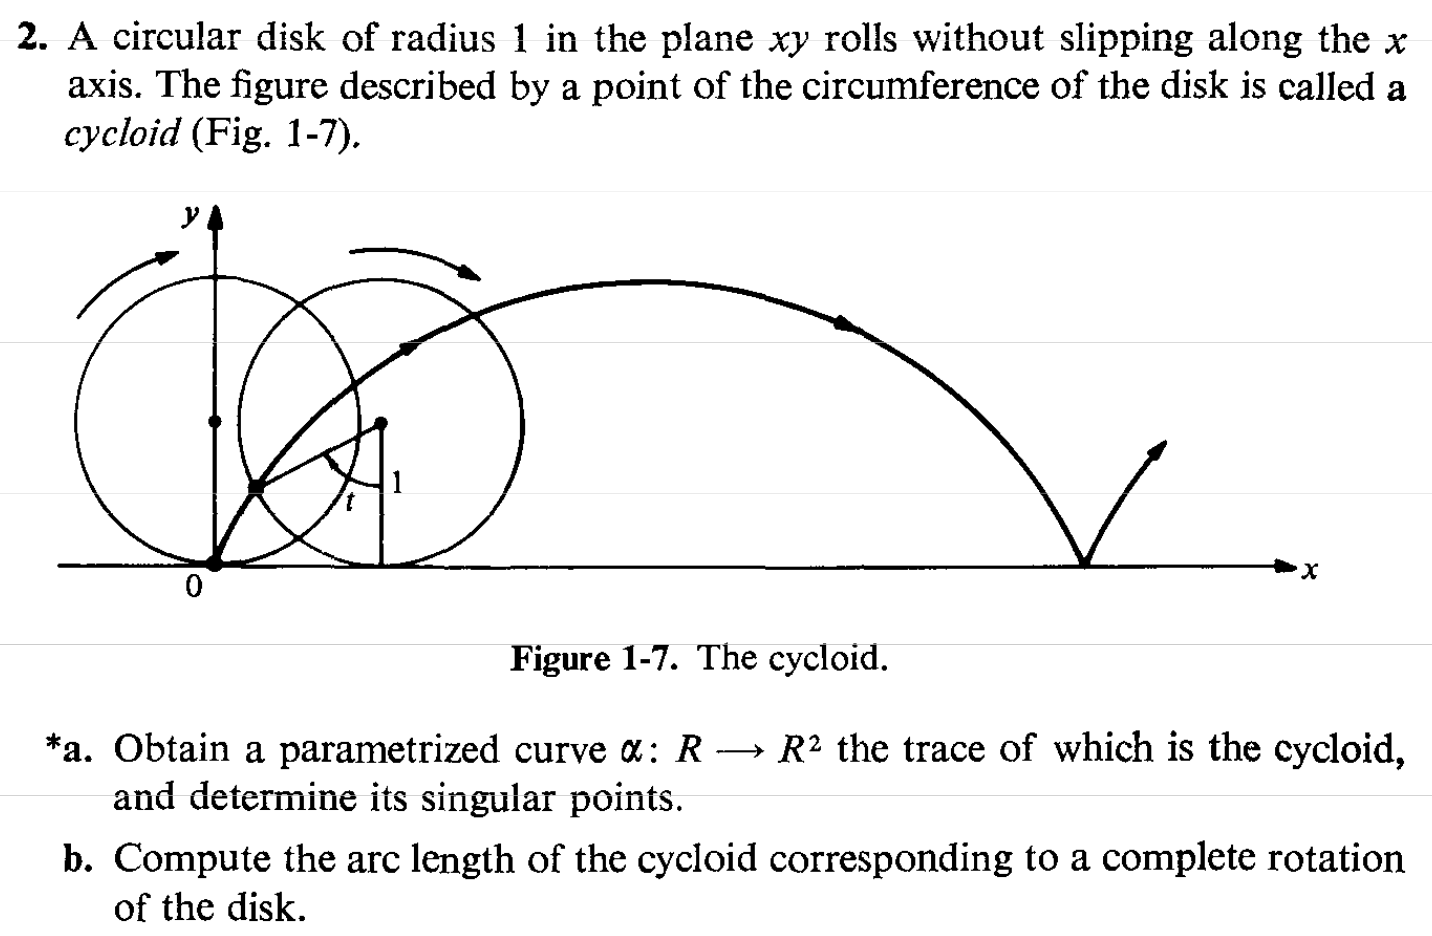
\includegraphics[height=10cm,width=18cm]{1.png}
\end{question}
\begin{proof}
The solution of the question \textbf{a} is 
\begin{align*}
\alpha (t)=(t-\sin t,1-\cos t)
\end{align*}
Compute 
\begin{align*}
\alpha'(t)=(1-\cos t,\sin t)
\end{align*}
and compute
\begin{align*}
\abso{\alpha '(t)}=\sqrt{1-2\cos t +\cos^2 t +\sin^2 t}  = \sqrt{2}\cdot \sqrt{1-\cos t}  
\end{align*}
This implies the singular points are 
\begin{align*}
  \set{2n\pi : n\inz}
\end{align*}


The solution of the question \textbf{b} is then 
\begin{align*}
\int_0^{2\pi} \abso{\alpha '(t)}dt&=\sqrt{2}\int_0^{2\pi} \sqrt{1-\cos t}dt \\
&=\sqrt{2} \int_{0}^{2\pi} \sqrt{2} \abso{\sin \frac{t}{2}}dt  \\
&=2\int_0^{2\pi}\abso{\sin \frac{t}{2}}dt\\
&=4 \int_{0}^{\pi}\sin (\frac{t}{2})dt\\
&=-8 \cos \frac{t}{2}\Big|_0^{\pi}
\end{align*}

\end{proof}
\begin{question}{1-3:4}{}
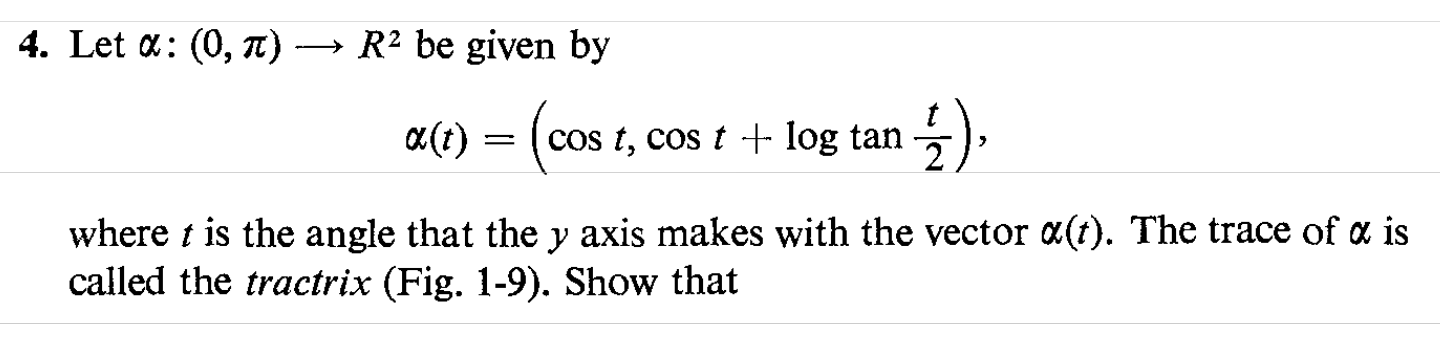
\includegraphics[height=4cm,width=18cm]{3.png}
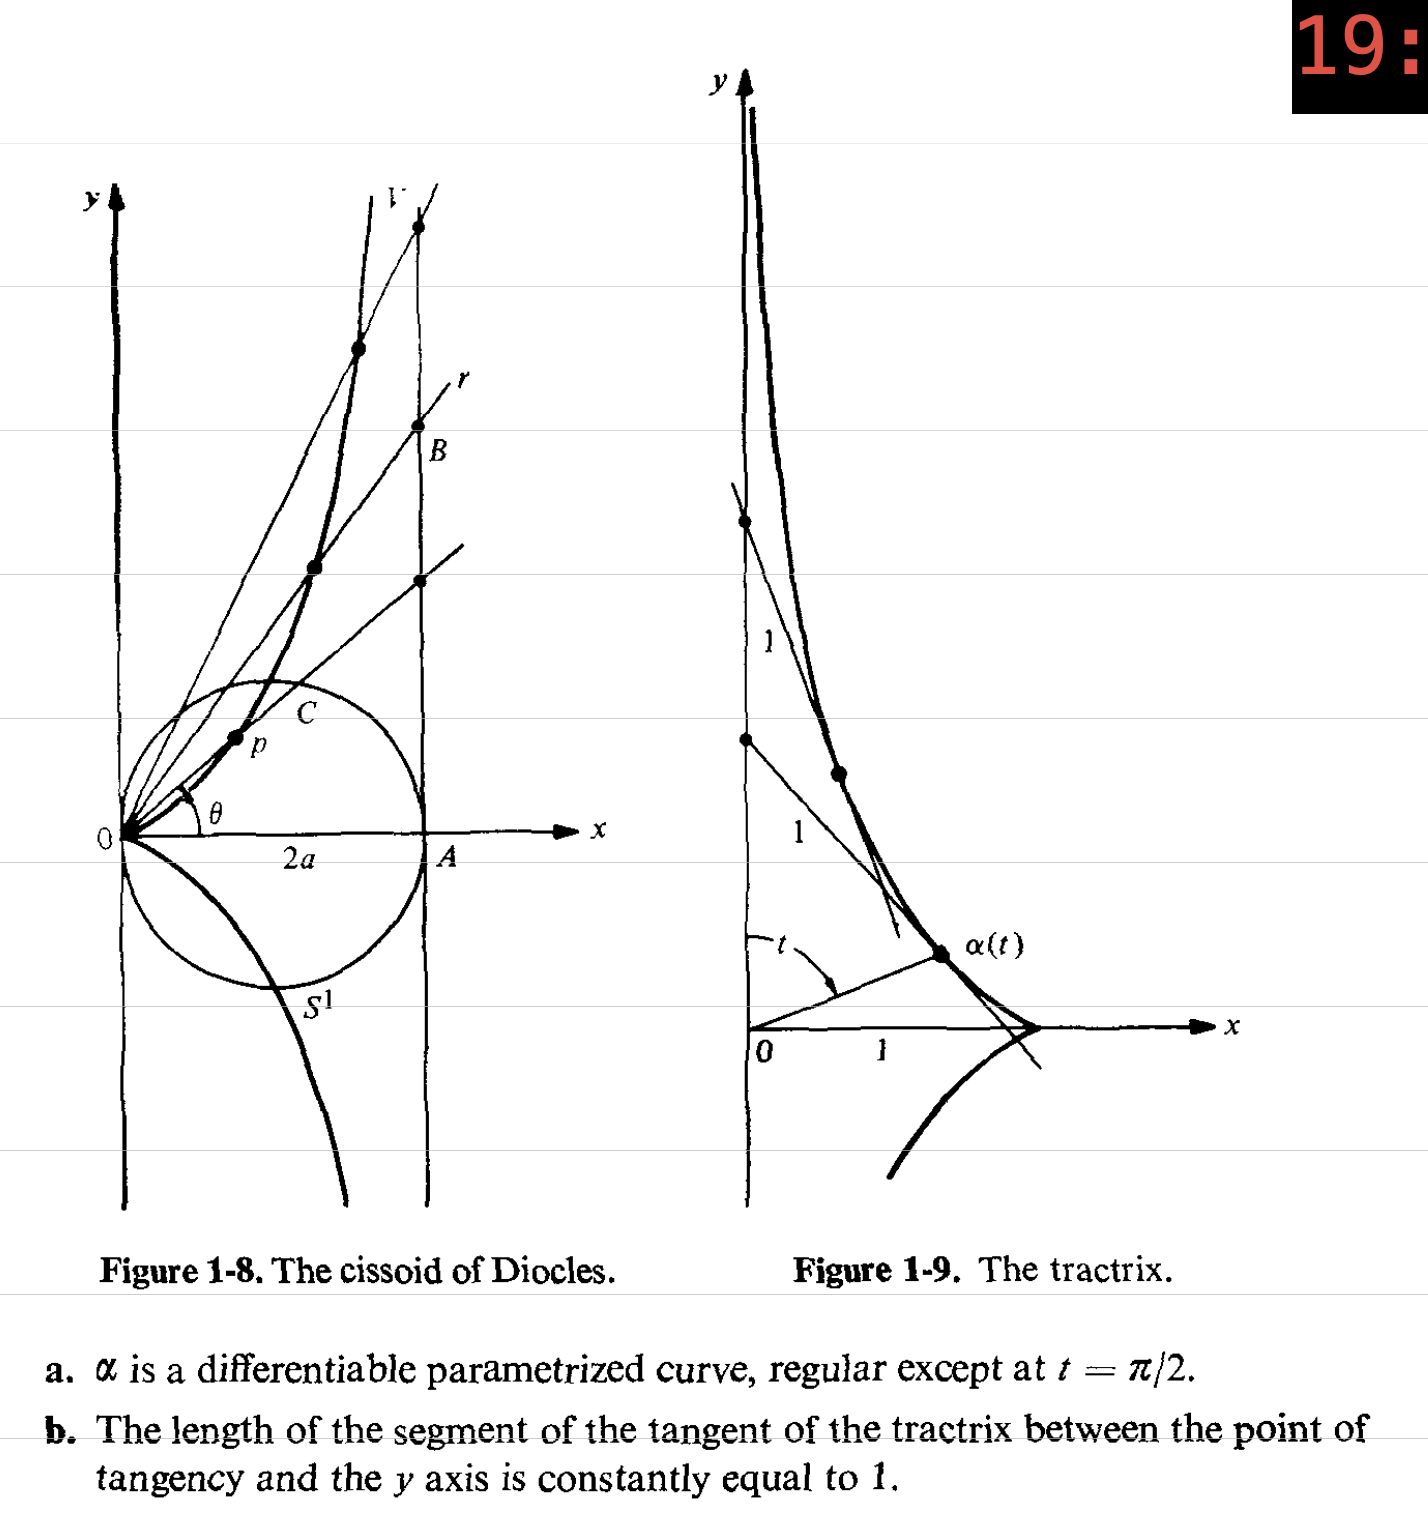
\includegraphics[height=18cm,width=18cm]{2.png}
Typo correction: $\alpha (t)=(\sin t,\cos t + \ln \tan \frac{t}{2})$
\end{question}
\begin{proof}
\textbf{(a)}

Notice that the interval $I$ is  $(0,\pi)$. It is clear that 
\begin{enumerate}[label=(\alph*)]
  \item $\sin t$ is smooth on $\R$
  \item $\cos t$ is smooth on $\R$
  \item $\ln t$ is smooth on $\R$
  $\tan \frac{t}{2}$ is smooth on $I$
\end{enumerate}
Then it follows that $\alpha $ is a differentiable curve.\\

Compute 
\begin{align*}
\alpha '(t)=(\cos t,- \sin t + \frac{1}{\tan \frac{t}{2}} \cdot \sec^2 \frac{t}{2}\cdot \frac{1}{2})
\end{align*}
Because $\cos t=\alpha '_1(t)$ is $0$ on  $I$ only when  $t=\frac{\pi}{2}$, we know $\alpha $ is regular on $I$ except possibly at  $t=\frac{\pi}{2}$.\\

Compute 
\begin{align*}
\alpha '(\frac{\pi}{2})=(0,-1+\frac{1}{1}\cdot 2 \cdot \frac{1}{2} )=(0,0)
\end{align*}
We now conclude $\alpha $ is regular on $I$ except  $\frac{\pi}{2}$. \\

\textbf{(b)}

A useful Identity give us 
\begin{align*}
\alpha '(t)=(\cos t,-\sin t+ \csc t)
\end{align*}
From the following facts
\begin{enumerate}[label=(\alph*)]
  \item the first argument of the segment is from $0$ to  $\sin t =\alpha (t)$
  \item $\alpha_x'(t)=\cos t$
  \item $\frac{\sin t}{\cos t}=\tan t$
\end{enumerate}
We conclude that the length of the segment is 
\begin{align*}
\abso{\tan t}\cdot \abso{\alpha '(t)}&= \abso{\tan t} \cdot \sqrt{\cos ^2 t + \sin^2 t - 2 \sin t \csc t + \csc ^2 t }\\
&=\abso{\tan t} \cdot \sqrt{1-2+\csc ^2 t}\\
&=\abso{\tan t } \cdot \sqrt{\csc ^2 t-1}=\abso{\tan t } \cdot  \sqrt{\cot ^2 t} =1
\end{align*}



\end{proof}
\begin{question}{}{}
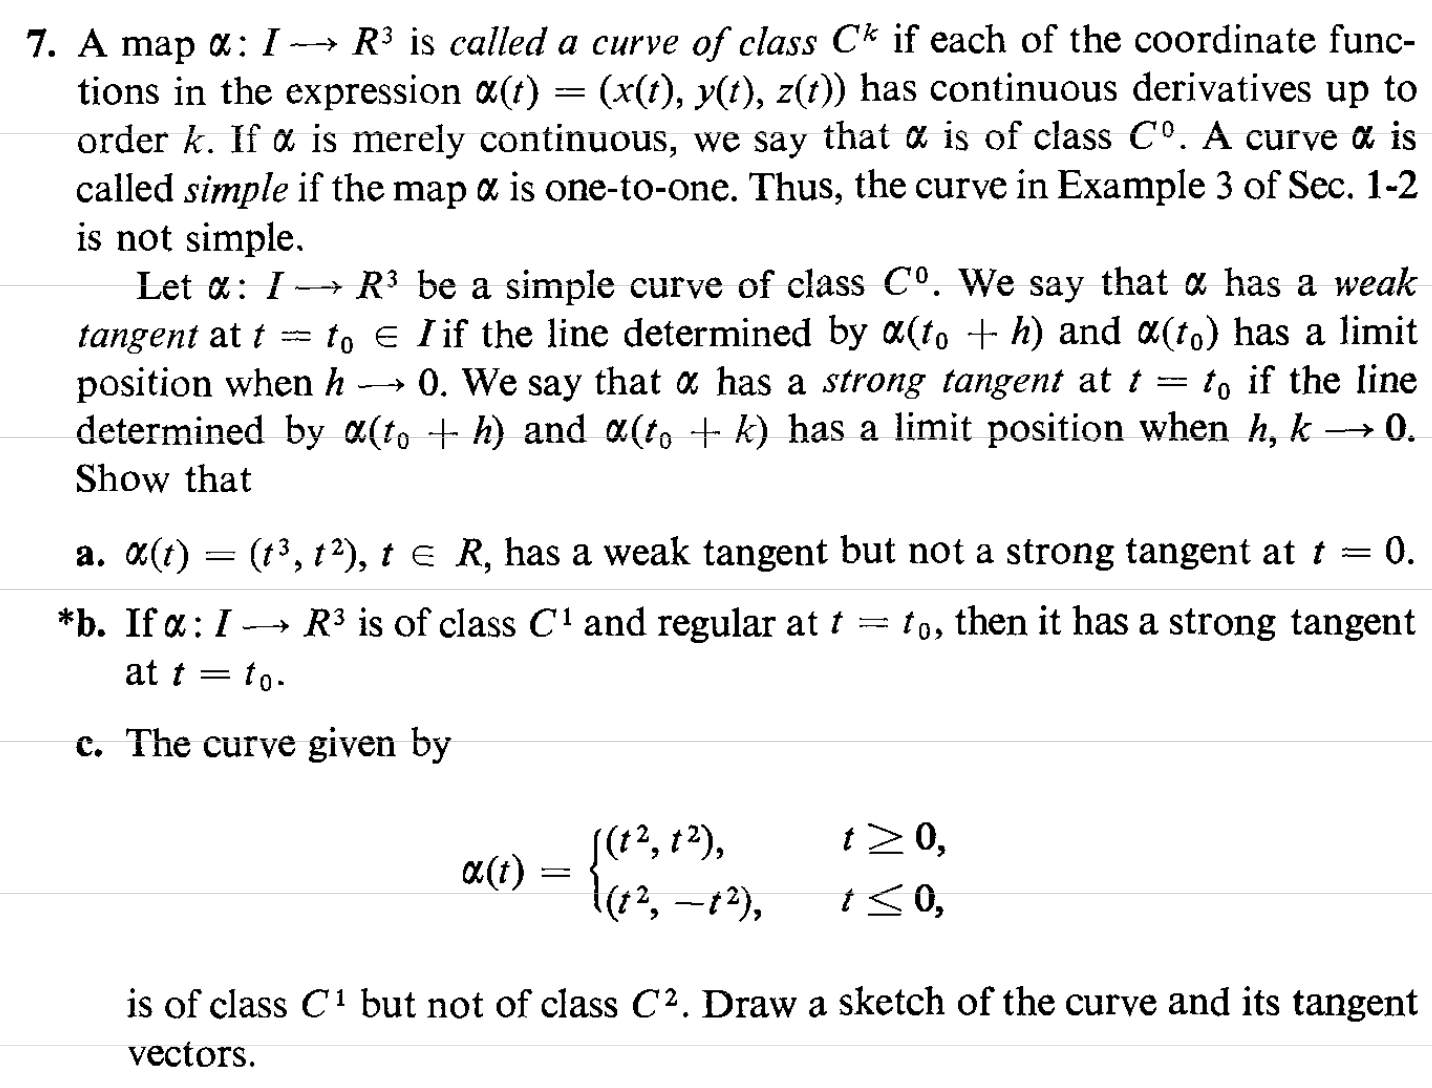
\includegraphics[height=14cm,width=18cm]{qu4}
\end{question}
\begin{proof}
\textbf{(a)}
Let $v=(0,1)$. Compute 
\begin{align*}
\frac{\alpha (t)-\alpha (0)}{\abso{\alpha (t)-\alpha (0)}}\cdot v=\frac{t^2}{\sqrt{t^6+t^4} }=\frac{1}{\sqrt{t^2+1} }\to 1\text{ as }t \to 1
\end{align*}
This implies $\alpha $ has a weak tangent at $t=0$. Now, if $\alpha $ has a strong tangent, we must have 
\begin{align*}
\frac{\alpha (h)-\alpha (-h)}{2h}\cdot v \to 1\text{ or }\to -1
\end{align*}
But this is clearly not the case as 
\begin{align*}
\frac{\alpha (h)-\alpha (-h)}{2h}\cdot v=0\text{ for all $h>0$ }
\end{align*}
So we have the conclusion that $\alpha $ has no strong tangent at $0$.\\


\textbf{(b)} 
By MVT, for each $h,k$ there exists a set of real numbers $\set{c_x,c_y,c_z}$ between $t+h$ and  $t+k$ such that 
 \begin{align*}
\frac{\alpha (t_0+h)-\alpha  (t_0+k)}{h-k}=\Big(x'(c_x),y'(c_y),z'(c_z) \Big)
\end{align*}
Then because 
\begin{align*}
h,k  \to 0 \implies t_0+h ,t_0+k \to t_0 \implies c_x,c_y,c_z \to t_0
\end{align*}
Then from the fact $\alpha $ is of class $C^1$ ($x',y',z'$ are all continuous), we can now deduce 
\begin{align}
\label{ahk}
\frac{\alpha (t_0+h)-\alpha (t_0+k)}{h-k}\to \alpha '(t_0)\text{ as $h,k \to 0$ }
\end{align}
Now, because $\alpha '(t_0)\neq 0$ as $\alpha $ is regular, we see 
\begin{align*}
\lim_{h,k\to 0}\frac{\alpha (t_0+h)-\alpha (t_0+k)}{h-k}\cdot \alpha '(t_0)= \abso{\alpha '(t_0)}^2
\end{align*}
This then implies 
\begin{align*}
\lim_{h,k\to 0}\frac{\alpha (t_0+h)-\alpha (t_0+k)}{\abso{\alpha (t_0+h)-\alpha (t_0+k)}}\cdot \frac{\alpha '(t_0)}{\abso{\alpha '(t_0)}}=1
\end{align*}
which implies the "strong tangent" must always converge to $\alpha '(t_0)$.\\

Notice that the last implication is backed by \myref{Equation}{ahk}\\


\textbf{(c)}\\

From 
\begin{align*}
\alpha (t)=\Big(t^2,\begin{cases}
  t^2& \text{ if $t\geq 0$ }\\
  -t^2& \text{ if $t\leq 0$ }
\end{cases} \Big)
\end{align*}
Compute 
\begin{align*}
\alpha '(t)=\Big(2t,\begin{cases}
  2t& \text{ if $t\geq 0$ }\\
  -2t& \text{ if $t\leq 0$ }
\end{cases} \Big)
\end{align*}
Notice that the derivative at $t=0$ is computed from definition instead of product rule.\\


Now, it is clear that $x',y'$ are continuous. This implies $\alpha  \in C^1$. Yet, we see $y'$ is not differentiable at  $t=0$. This implies  $\alpha \not \in C^2$.\\

The sketch: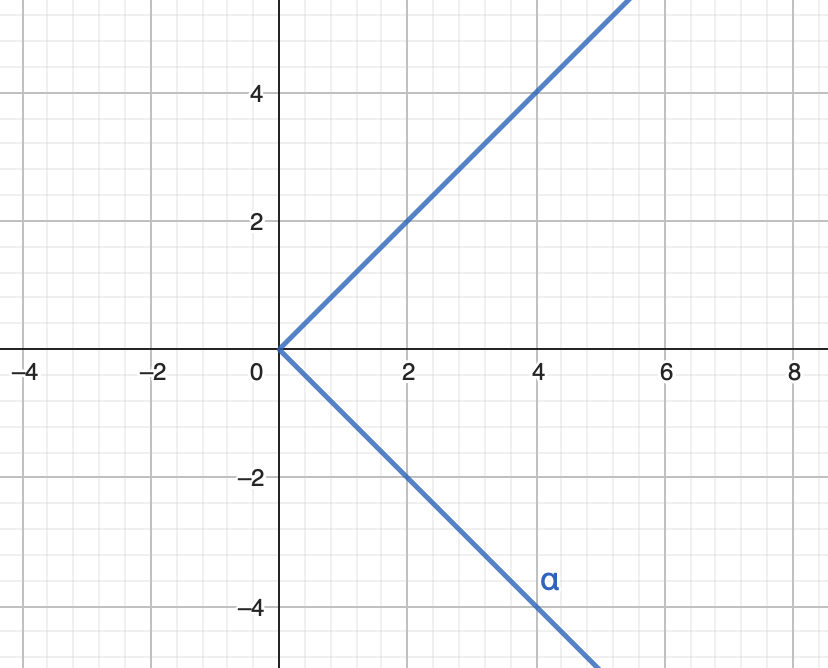
\includegraphics[height=8cm,width=15cm]{qsp}
\end{proof}
\begin{question}{}{}
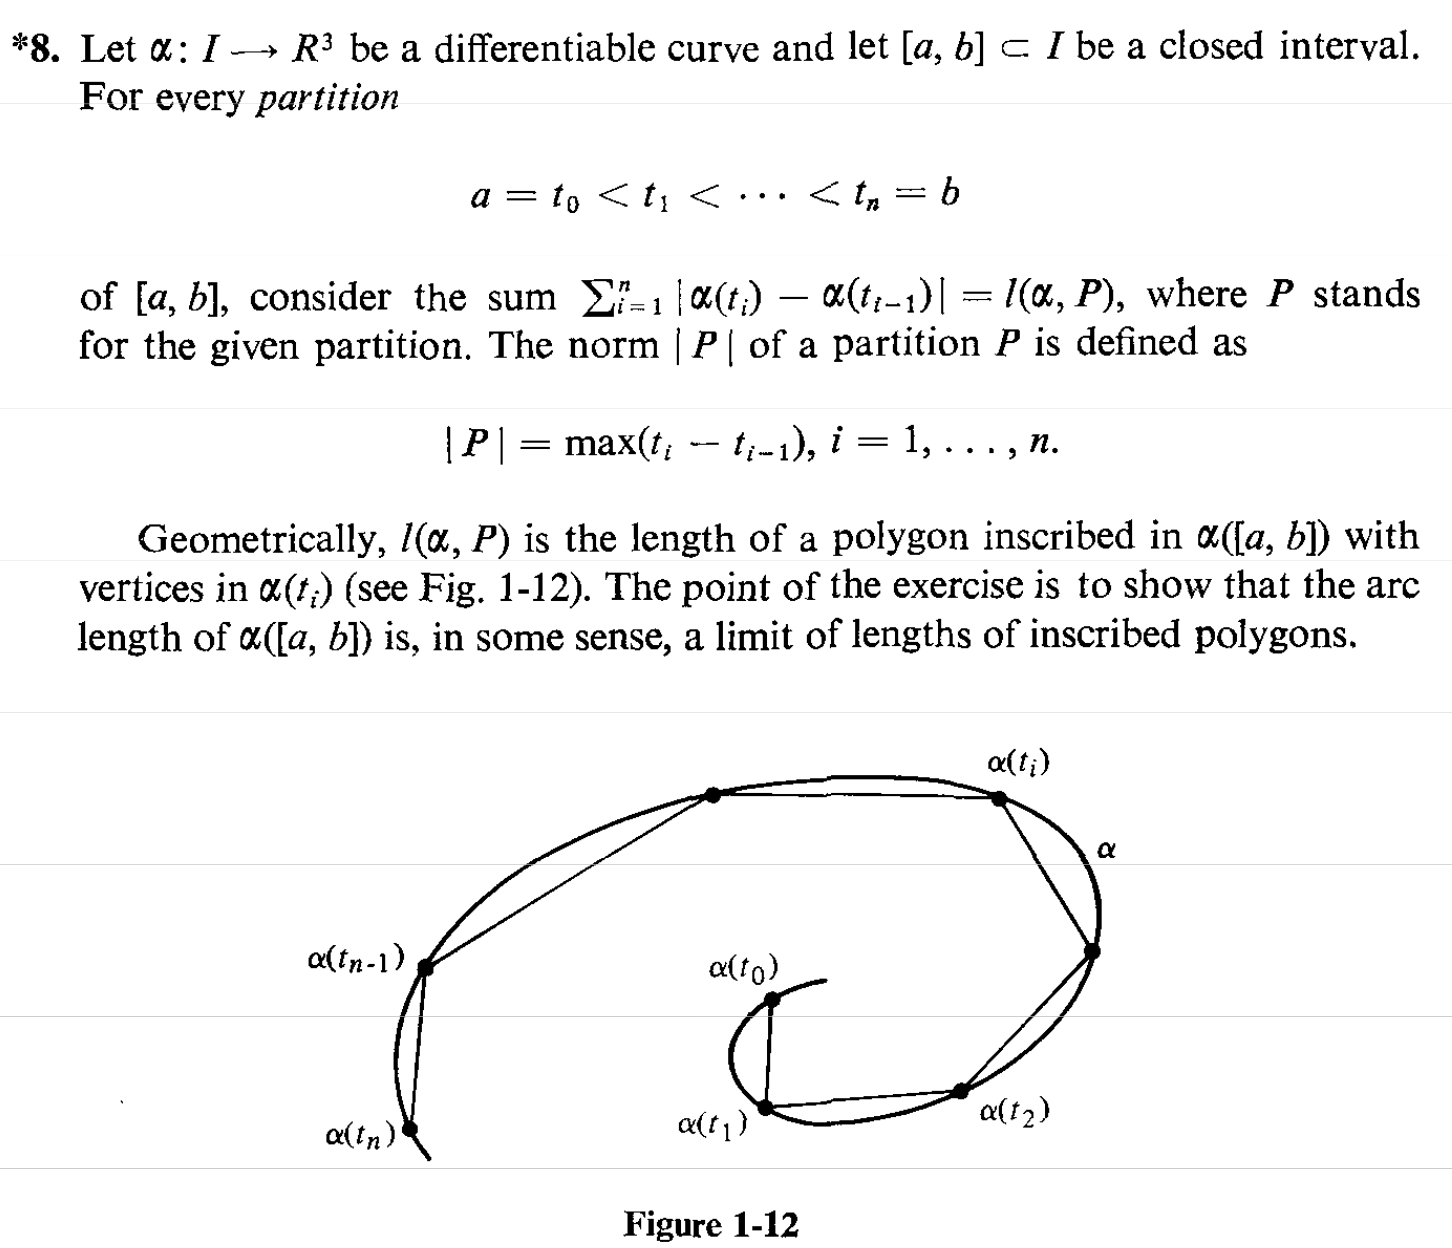
\includegraphics[height=15cm,width=18cm]{qu8}
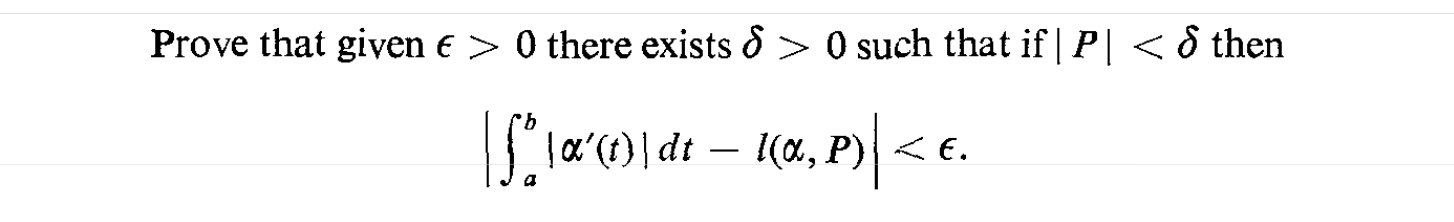
\includegraphics[height=3cm,width=18cm]{qu7}
\end{question}
\begin{proof}
We first prove 
\begin{align*}
\vi{\int_a^b \abso{\alpha '(t)}dt \geq  l(\alpha ,P)}
\end{align*}
By FTC, we have
\begin{align*}
  \abso{\alpha (t_i)-\alpha (t_{i-1})}&=\abso{\int_{t_{i-1}}^{t_i} \alpha '(t)dt}\\
&\leq \int_{t_{i-1}}^{t_i} \abso{\alpha '(t)}dt 
\end{align*}
This then implies 
\begin{align*}
l(\alpha ,P)=\sum \abso{\alpha (t_i)-\alpha (t_{i-1})}\leq \sum \int_{t_{i-1}}^{t_i}\abso{\alpha '(t)}dt=\int_a^b \abso{\alpha '(t)}dt \vdone
\end{align*}
We have reduced the problem into 
\begin{align*}
\blue{\text{ finding $\delta$ such that }\forall P: \abso{P}<\delta , \int_a^b \abso{\alpha '(t)}dt - l(\alpha ,P)<\epsilon }
\end{align*}


Because $\alpha '$ is uniformly continuous on $[a,b]$ ($\because$ continuous function on compact domain is uniformly continuous), we know there exists $\delta ' $ such that 
\begin{align*}
\abso{\alpha '(s)-\alpha '(t)}< \frac{\epsilon }{2(b-a)}\text{ if $\abso{s-t}<\delta'$ }
\end{align*}
We claim 
\begin{align*}
\blue{\text{ such $\delta'$ works }}
\end{align*}
Let $\abso{P}<\delta$, and let $s_i \in [t_{i-1},t_i]$. Because $\abso{s_i-t_i}<\delta$, we have
\begin{align}
\label{siti}
\abso{\alpha '(s_i)-\alpha '(t_i)}<\frac{\epsilon}{2(b-a)}
\end{align}
This give us 
\begin{align*}
\abso{\alpha '(s_i)}<\abso{\alpha '(t_i)} + \frac{\epsilon}{2(b-a)}
\end{align*}
Now, we can deduce 
\begin{align*}
  \int_{t_{i-1}}^{t_i} \abso{\alpha '(s)}ds&\leq   \abso{\alpha '(t_i)}\Delta t_i+ \frac{\epsilon }{2(b-a)}\Delta t_i\\
  &=\int_{t_{i-1}}^{t_i}\abso{\alpha '(t_i)}dt + \frac{\epsilon}{2(b-a)}\Delta t_i\\
 &=\abso{\int_{t_{i-1}}^{t_i} \alpha '(t_i)dt}+ \frac{\epsilon }{2(b-a)}\Delta t_i\\
  &=\abso{\int_{t_{i-1}}^{t_i} \alpha' (t_i)-\alpha '(t)dt + \int_{t_{i-1}}^{t_i} \alpha '(t)dt }+ \frac{\epsilon}{2(b-a)}\Delta t_i \\
  &\leq  \abso{\int_{t_{i-1}}^{t_i} \alpha '(t_i)-\alpha' (t)dt}+ \abso{\int_{t_{i-1}}^{t_i} \alpha '(t)dt}+\frac{\epsilon}{2(b-a)}\Delta t_i \\
  &\leq \frac{\epsilon}{2(b-a)}\Delta t_i + \abso{\alpha (t_i)-\alpha (t_{i-1})}+\frac{\epsilon}{2(b-a)}\Delta t_i\\
  &=\abso{\alpha (t_i)-\alpha (t_{i-1})}+ \frac{\epsilon }{b-a}\Delta t_i
\end{align*}
Notice that the last inequality follows from \myref{Equation}{siti}. The long deduction above then give us 
\begin{align*}
  \int_{a}^b \abso{\alpha '(t)}dt&\leq \sum \abso{\alpha (t_i)-\alpha (t_{i-1})}+ \frac{\epsilon}{b-a} (b-a)\\
&=l(\alpha ,P)+\epsilon 
\end{align*}
Then we have 
\begin{align*}
\int_a^b \abso{\alpha '(t)}dt -l(\alpha ,P)\leq \epsilon \bdone
\end{align*}
\end{proof}
\begin{question}{}{}
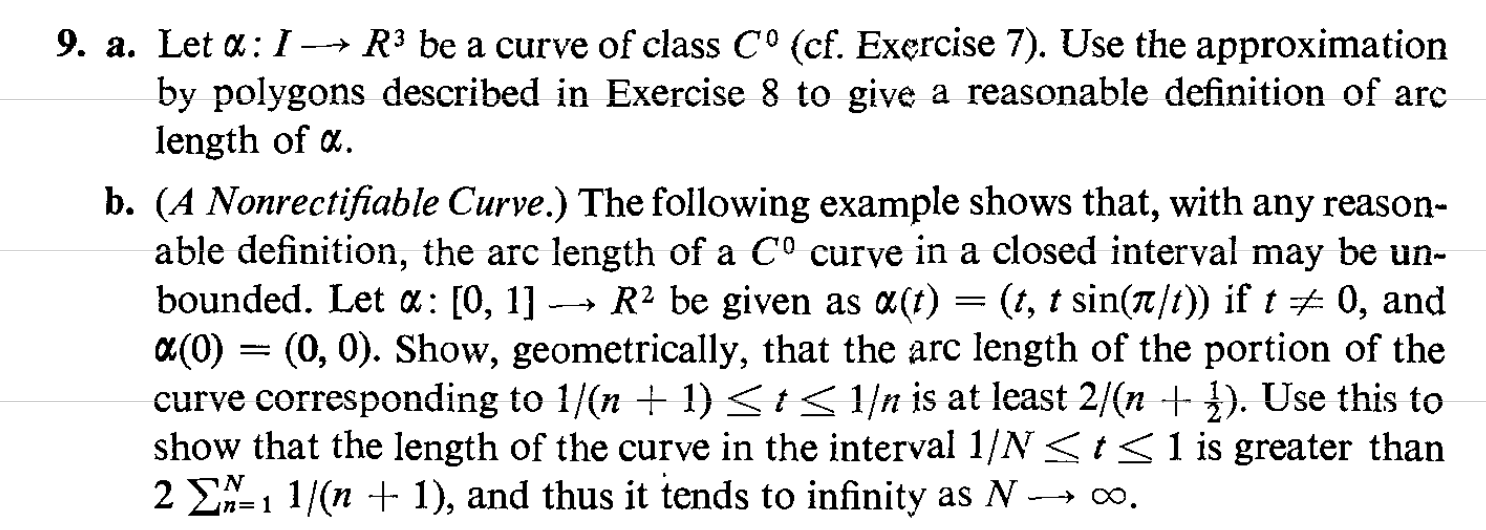
\includegraphics[height=7cm,width=18cm]{qu6}
\end{question}
\begin{proof}
\textbf{(a)} 
Suppose $I=[a,b]$. Define arc length by 
\begin{align*}
\sup_{P} l(P,\alpha )\text{ where $\sup $ runs over all partition $P$ of $[a,b]$  }
\end{align*}

\textbf{(b)}\\

Geometrically, we know the arc length of the portion of the curve corresponding to $t \in [\frac{1}{n+1},\frac{1}{n}]$ must be greater than 
\begin{align}
\label{19b}
\abso{\alpha \big(\frac{1}{n}\big)-\alpha \big(\frac{1}{n+\frac{1}{2}}\big)}+\abso{\alpha \big(\frac{1}{n+1} \big)-\alpha \big(\frac{1}{n+\frac{1}{2}} \big)}
\end{align}
WOLG of $n$ being odd or even, Compute 
\begin{align*}
\abso{\alpha \big(\frac{1}{n} \big)-\alpha \big(\frac{1}{n+\frac{1}{2}} \big)}&=\abso{(\frac{1}{n},0)-(\frac{1}{n+\frac{1}{2}},\frac{1}{n+\frac{1}{2}})}\\
&=\sqrt{\big(\frac{1}{n}-\frac{1}{n+\frac{1}{2}} \big)^2 +\big(\frac{1}{n+\frac{1}{2}} \big)^2} \\
&=\sqrt{\frac{1}{n^2}-\frac{4}{n(2n+1)}+\frac{8}{(2n+1)^2}} \\
&=\sqrt{\frac{(2n+1)^2-4n(2n+1)+8n^2}{n^2(2n+1)^2}} \\
&=\sqrt{\frac{4n^2+1}{n^2(2n+1)^2}}\\
&=\frac{\sqrt{4n^2+1} }{n(2n+1)}\geq \frac{\sqrt{4n^2} }{n(2n+1)}=\frac{2}{2n+1}
\end{align*}
and compute 
\begin{align*}
\abso{\alpha \big(\frac{1}{n+\frac{1}{2}} \big)-\alpha \big(\frac{1}{n} \big)}&=\abso{(\frac{1}{n+\frac{1}{2}},\frac{1}{n+\frac{1}{2}})-(\frac{1}{n+1},0)}\\
&=\sqrt{\big(\frac{1}{n+1}-\frac{1}{n+\frac{1}{2}} \big)^2 + \big(\frac{1}{n+\frac{1}{2}} \big)^2} \\
&=\sqrt{\frac{1}{(n+1)^2}-\frac{4}{(n+1)(2n+1)}+\frac{8}{(2n+1)^2}}\\
&=\sqrt{\frac{(2n+1)^2 -4(n+1)(2n+1)+8(n+1)^2}{(n+1)^2(2n+1)^2}}\\
&=\sqrt{\frac{4n^2+8n+5}{(n+1)^2(2n+1)^2}}\\
&\geq \frac{\sqrt{4n^2+8n+4} }{(n+1)(2n+1)}=\frac{2}{2n+1}
\end{align*}
From the computation and \myref{Equation}{19b}, it is now clear that the arc length of the portion of the curve corresponding to $ t \in [\frac{1}{n+1},\frac{1}{n}]$ is at least $\frac{2}{n+\frac{1}{2}}$. With simple addition, this then implies the arc length of the curve in the interval $[\frac{1}{N},1]$ is at least 
\begin{align*}
  \sum_{n=1}^{N-1} \frac{2}{2n+1}=2 \sum_{n=1}^{N-1}\frac{1}{2n+1}
\end{align*}
The number is clearly greater than 
\begin{align*}
2 \sum_{n=1}^{N-1}\frac{1}{2n+2}
\end{align*}
which equals to 
\begin{align*}
\sum_{n=1}^{N-1}\frac{1}{n+1}
\end{align*}
The series diverge to $+\infty$ as $N$ to  $\infty$. 
\end{proof}
\begin{theorem}
\label{IDP}
\textbf{(Integrating the Dot Product)} Given a curve $u:[a,b]\rightarrow \R^n$ and a vector $v \in\R^n$, suppose 
\begin{enumerate}[label=(\alph*)]
  \item $u$ is differentiable on $(a,b)$ 
  \item $u$ is continuous on  $[a,b]$
\end{enumerate}
We have 
\begin{align*}
\int_a^b u'(t)\cdot v dt=
\Big(\int_a^b u'(t)dt \Big)\cdot v= \big(u(b)-u(a) \big)\cdot v
\end{align*}
\end{theorem}
\begin{proof}
\begin{align*}
\int_a^b u'(t)\cdot vdt&=\int_a^b \sum_{k=1}^n u'_k(t)\cdot v_k dt \\
&=\sum_{k=1}^n  \int_a^b u'_k(t)\cdot v_k dt\\
&=\sum_{k=1}^n v_k \int_a^b u'_k(t)dt\\
&=v\cdot \Big(\int_a^b u'(t)dt \Big)
\end{align*}
\end{proof}
\begin{question}{}{}
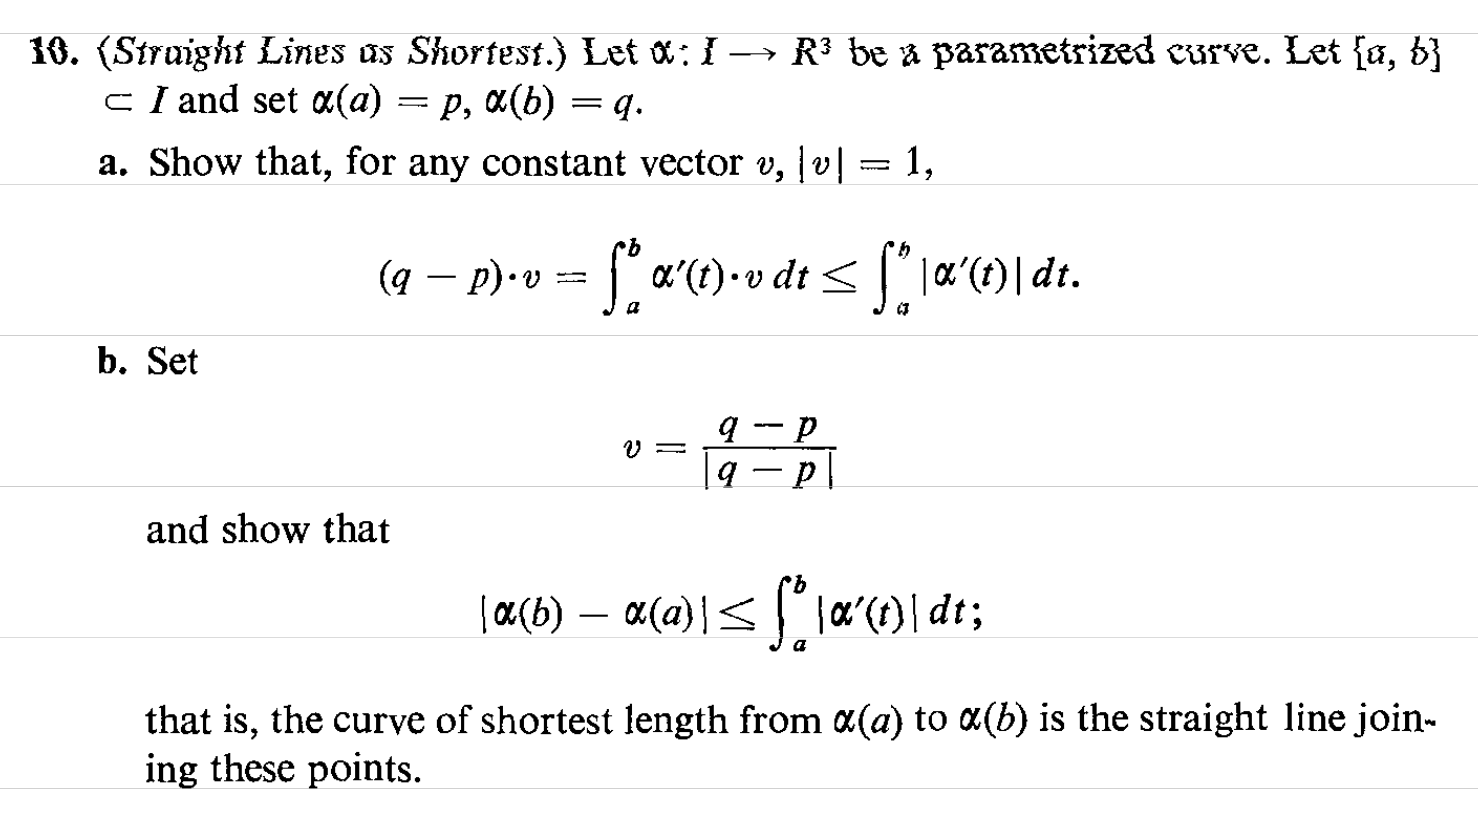
\includegraphics[height=10cm,width=18cm]{qu5}
\end{question}
\begin{proof}
\textbf{(a)}\\


The first equality 
\begin{align*}
  (q-p)\cdot v=\int_a^b \alpha '(t)\cdot vdt
\end{align*}
follows directly from \myref{Theorem}{IDP}.\\

Now, by Cauchy-Schwarz inequality, we have 
\begin{align*}
  \abso{\alpha '(t)\cdot v} \leq \abso{\alpha '(t)}\cdot \abso{v}
\end{align*}
This then give us 
\begin{align*}
\alpha '(t)\cdot v\leq \abso{\alpha '(t)\cdot v}\leq \abso{\alpha '(t)}\cdot \abso{v}=\abso{\alpha '(t)}
\end{align*}
We now have 
\begin{align*}
\int_a^b \alpha '(t)\cdot v \leq \abso{\alpha '(t)}dt
\end{align*}
as desired.\\

\textbf{(b)}

The first inequality tell us that if $v$ is a constant and $\abso{v}=1$, we have 
\begin{align*}
  (q-p)\cdot v \leq \int_a^b \abso{\alpha '(t)}dt
\end{align*}
If $v=\frac{q-p}{\abso{q-p}}$, it is clear that $v$ is a constant and  $\abso{v}=1$, and at the same time, we have 
\begin{align*}
  (q-p)\cdot v=\frac{(q-p)\cdot (q-p)}{\abso{q-p}}=\frac{\abso{q-p}^2}{\abso{q-p}}=\abso{q-p}
\end{align*}
We now have 
\begin{align*}
\abso{q-p}=(q-p)\cdot v \leq \int_a^b \abso{\alpha '(t)}dt
\end{align*}
from the first inequality 
\end{proof}
\begin{question}{}{}
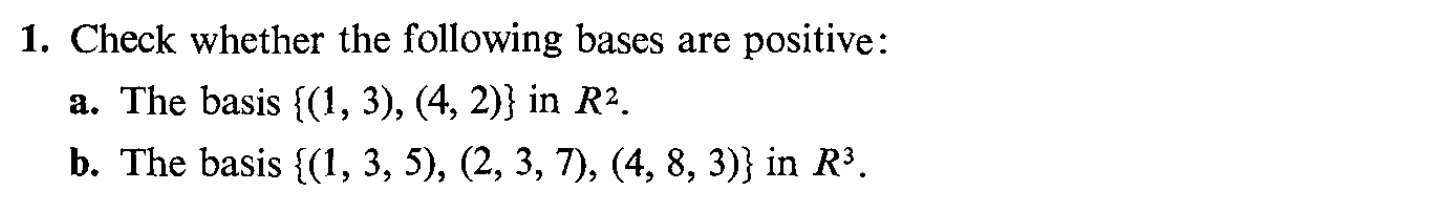
\includegraphics[height=2cm,width=18cm]{qu9}
\end{question}
\begin{proof}
Compute 
\begin{align*}
\begin{vmatrix} 
  1 & 4 \\
  3 & 2
\end{vmatrix}=-10
\end{align*}
and compute 
\begin{align*}
\begin{vmatrix}
  1& 2 & 4 \\
  3 & 3 & 8 \\
  5 & 7 & 3
\end{vmatrix}=-9
\end{align*}
Both bases are negatively oriented. 
\end{proof}
\begin{question}{}{}
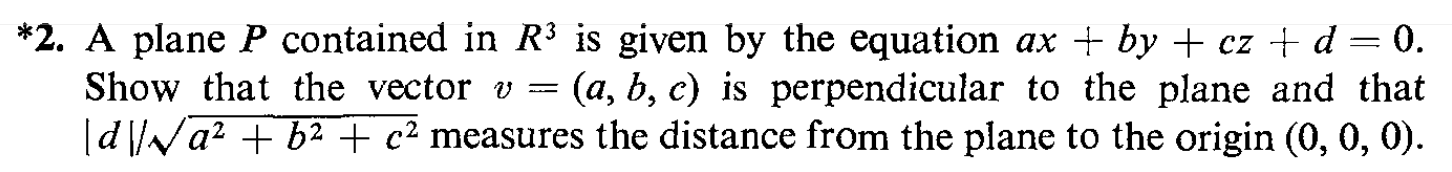
\includegraphics[height=2cm,width=18cm]{qu10}
\end{question}
\begin{proof}
Arbitrarily pick two points $u,w$ in  $P$. We wish to show 
\begin{align*}
  \vi{v\cdot (u-w)=0}
\end{align*}
Because $v=(a,b,c)$ and 
\begin{align*}
\begin{cases}
  au_1+b u_2+cu_3=-d
  aw_1+b w_2+cw_3=-d
\end{cases}
\end{align*}
We see
\begin{align*}
v\cdot (u-w)&= a(u_1-w_2)+b(u_2-w_2)+c(u_3-w_2)\\
&=(-d)-(-d)=0\vdone
\end{align*}
To measure the distance between $P$ and the origin, we wish to find a vector $u$ such that  $u\perp P$ and $u \in P$. We know that $u$ must be linearly dependent with  $v=(a,b,c)$, since the dimension of  $P^\perp$ is $1$. Then, we can write
\begin{align*}
u=c_0(a,b,c)\text{ for some $c_0\inr$ }
\end{align*}
Because $u \in P$, we know 
\begin{align*}
c_0a^2+c_0b^2+c_0c^2+d=0
\end{align*}
This tell us 
\begin{align*}
c_0=\frac{-d}{a^2+b^2+c^2}
\end{align*}
We now see that the distance $\abso{u}$ between $P$ and origin is 
\begin{align*}
\abso{u}=\abso{c_0}\cdot \sqrt{a^2+b^2+c^2}= \frac{\abso{d}}{\sqrt{a^2+b^2+c^2} }
\end{align*}

\end{proof}
\begin{question}{}{}
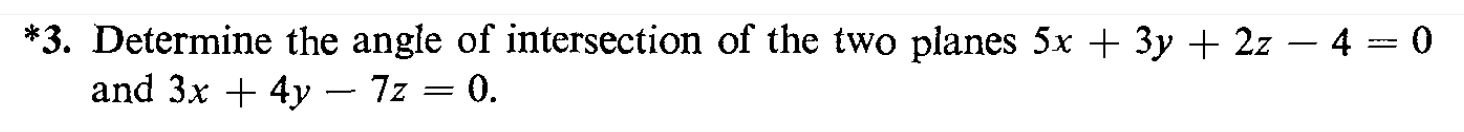
\includegraphics[height=2cm,width=18cm]{qu11}
\end{question}
\begin{proof}
From last question, we know the two vectors $u,v$ that are respectively perpendicular to  $P:5x+3y+2z-4=0$ and  $Q:3x+4y-7z=0$ respectively have the direction 
 \begin{align*}
   (5,3,2)\text{ and }(3,4,-7)
\end{align*}
Then, we see the angle of the intersection are 
\begin{align*}
\arccos \frac{5\cdot 3+3\cdot 4 +2 \cdot (-7)}{\sqrt{5^2+3^2+2^2} \sqrt{3^2+4^2+7^2} }=\arccos \frac{13}{\sqrt{38}\sqrt{71}  }
\end{align*}
Notice that this angle is smaller than $\frac{\pi}{2}$ as we intend it to be. 
\end{proof}
\begin{question}{}{}
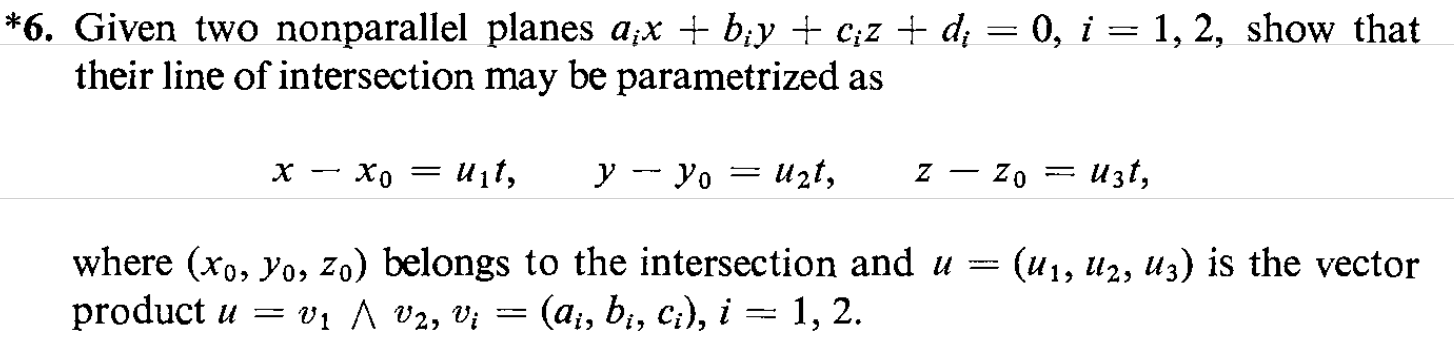
\includegraphics[height=4cm,width=18cm]{qu12}
\end{question}
\begin{proof}
Let $v=(x,y,z)$ be a point on the line of intersection.  We see the vector  $v-(x_0,y_0,z_0)$ lies on both planes, and thus must be perpendicular to $(a_1,b_1,c_1)=v_1$ and $(a_2,b_2,c_2)=v_2$ thus satisfying 
\begin{align*}
v-(x_0,y_0,z_0)=tv_1\times v_2=tu\text{ for some $t\inr$ }
\end{align*}
sine in $\R^3$, the only direction perpendicular to both  $v_1,v_2$ is  $v_1\times v_2$. We can rewrite the above equation of course into 
\begin{align*}
x-x_0=u_1t,y-y_0=u_2t,z-z_0=u_3t
\end{align*}
\end{proof}
\section{Fundamental Theorem of Local Curves}
\begin{mdframed}
In this section, by an \textbf{orthogonal transformation} we mean a linear transformation $M$ from  $\big(V,\langle \cdot,\cdot\rangle_V  \big)$ to $\big(W,\langle \cdot,\cdot\rangle_W  \big)$ such that 
\begin{align*}
\hspace{3cm}\langle v,w\rangle_V =\langle Mv,Mw\rangle_W\hspace{2cm}(v,w \in V)
\end{align*}
By a \textbf{rigid motion} $M$, we mean an orthogonal transformation from $\R^3$ to  $\R^3$ such that 
\begin{align*}
\text{det}\big([M]_{\set{e_1,e_2,e_3}} \big)>0
\end{align*}
\end{mdframed}
\begin{theorem}
\textbf{(Fundamental Theorem of Local Curves: Uniqueness Part 1)} Given an $\underline{\text{open}}$ interval $I \subseteq \R$, a parametrized by arc-length curve $\alpha :I \rightarrow \R^3$ with positive curvature, a rigid motion $M$ and a vector  $c \inr^3$, we see that the function  $\beta : I \rightarrow \R^3 $ defined by 
\begin{align*}
\beta (s)=(M \circ \gamma )(s)+c
\end{align*}
is a curve parametrized by arc-length such that 
\begin{align*}
\alpha \text{ and }\beta \text{ has the same curvature and torsion on all $s \in I$ }
\end{align*}
\end{theorem}
\begin{proof}
We first have to prove 
\begin{align*}
\vi{\beta :I\rightarrow \R^3\text{ is parametrized by arc-length }}
\end{align*}
Fix $s \in I$. We have to prove 
\begin{align*}
\vi{\abso{\beta '(s)}=1}
\end{align*}
Compute 
\begin{align*}
\abso{\beta '(s)}&=\abso{(M\circ \gamma )'(s)}\\
&=\abso{}\vdone
\end{align*}
We now prove 
\begin{align*}
\blue{\beta '(s)}
\end{align*}

Because we have the identity 
\begin{align*}
\kappa (s)=\abso{\alpha ''(s)}\text{ and }\tau (s)=-\frac{(\alpha '\times \alpha '')\cdot \alpha '''}{\kappa^2}
\end{align*}
\end{proof}
\begin{theorem}
\label{FTLCU}
\textbf{(Fundamental Theorem of Local Curves: Uniqueness Part 2)} Given an $\underline{\text{open}}$ interval $I \subseteq \R$ and two parametrized by arc-length curves $\alpha ,\overline{\alpha }:I\rightarrow \R^3$ such that 
\begin{align*}
\hspace{3cm}\kappa(s)=\overline{\kappa}(s)\text{ and }\tau(s)=\overline{\tau}(s)\hspace{2cm}(s \in I)
\end{align*}
Then there exists an rigid motion $M$ and a vector  $c \inr^3$ such that 
\begin{align*}
\hspace{3cm}\alpha (s)=M\big(\overline{\alpha }(s) \big)+c\hspace{2cm}(s \in I)
\end{align*}
\end{theorem} 
\begin{proof}
Fix distinct $s_0\in I$. We first have to 
\begin{align*}
  \vi{\text{ find a rigid motion $M:\R^3\rightarrow \R^3$ and some vector $c\inr^3$ }}\\
\vi{\text{ such that $\begin{cases}
  \alpha (s_0)=(M\circ \overline{\alpha })(s_0)+c\\
  T(s_0)=M\circ \overline{T}(s_0)\\
  N(s_0)=M\circ \overline{N}(s_0)\\
  B(s_0)=M\circ \overline{B}(s_0)
\end{cases}\vdone$}}
\end{align*}
Now, express 
\begin{align*}
T_M(s)=\text{ normal tangent of }M\circ \overline{\alpha }+c\text{ at $s$ }
\end{align*}
We show 
\begin{align*}
\blue{\begin{cases}
  T_M=T\\
  N_M=N\\
  B_M=B
\end{cases}\text{ on $I$ }}
\end{align*}
By Frenet Formula, compute 
\begin{align*}
&\frac{1}{2}\frac{d}{ds}\Big(\abso{T-T_M}^2+ \abso{N-N_M}^2+\abso{B-B_M}^2 \Big)\\
=&\frac{1}{2}\frac{d}{ds}\Big(\sum_{X=T,N,B} (X-X_M)\cdot (X-X_M)\Big)\\
=&\sum_{X=T,N,B} (X-X_M)'\cdot (X-X_M)\\
=&\sum_{X=T,N,B} (X'-X_M')\cdot (X-X_M)\\
=&(T'-T'_M)\cdot (T-T_M)+(N'-N'_M)\cdot (N-N_M)+(B'-B_M')\cdot (B-B_M)\\
 &\\
=&(\kappa N'-\kappa N'_M)\cdot (T-T_M)\\
+\Big)&\big(-\kappa T-\tau B+\kappa T_M'+\tau BT'_M \big)\cdot (N-N_M)\\
+\Big)& \big(\tau N-\tau N_M\big)\cdot (B-B_M)\hspace{1cm}(\because \text{ Frenet Formula and $\alpha ,\alpha _M$ same curvature and torsion})\\
=&0\hspace{1cm}(\because\text{ Elimination })
\end{align*}
We now know 
\begin{align*}
\abso{T-T_M}^2+\abso{N-N_M}^2+\abso{B-B_M}^2\text{ is a constant }
\end{align*}
Moreover, because by our setting  
\begin{align*}
\Big( \abso{T-T_M}^2+\abso{N-N_M}^2+\abso{B-B_M}^2\Big)(s_0)=0
\end{align*}
We know 
\begin{align*}
\hspace{3cm}\abso{T-T_M}^2+\abso{N-N_M}^2+\abso{B-B_M}^2=0\hspace{1cm}(s \in I)
\end{align*}
This implies 
\begin{align*}
\begin{cases}
  T=T_M\\
  N=N_M\\
  B=B_M
\end{cases}\text{ on $I\bdone$ }
\end{align*}
Because both  $\alpha $ and $\alpha _M$ are parametrized by arc-length and $\alpha (s_0)=\alpha _M(s_0)$, we now see 
\begin{align*}
\hspace{2cm}\alpha (s)=\int_{s_0}^s T(x)dx+ \alpha (s_0)=\int_{s_0}^s T_M(x)dx+ \alpha_M(s_0)=\alpha_M(s)\hspace{1cm}(s \in I)
\end{align*}
This finish the proof. 
\end{proof}

\section{Isoperimetric Inequality}
\begin{mdframed}
In this section, by \textbf{a closed plane curve}, we mean a regular parametrized curve $\alpha :[a,b]\rightarrow \R^2$ such that 
\begin{align*}
\alpha^{(n)}(a)=\alpha^{(n)}(b)\text{ for all $n\inz_0^+$ }
\end{align*}
If we say a closed plane curve $\alpha :[a,b]\rightarrow \R^2$ is \textbf{simple}, we mean 
\begin{align*}
\alpha (t_1)\neq \alpha (t_2)\text{ for all distinct pair $(t_1,t_2) \subseteq [a,b]$ except $(a,b)$}
\end{align*}
A closed plane curve must divide $\R^2$ into two separate subsets, in the sense that  $\R^2 \setminus \alpha \big[[a,b] \big]$ has two connected component. The one connected component that has finite area in the sense of Lebesgue outer measure is called the \textbf{interior} of the $\alpha $. If the interior is always on the left side of $\alpha $, we say $\alpha $ is \textbf{positively oriented}, in other words, $\alpha $ runs counter clockwise.
\end{mdframed}
\begin{theorem}
\textbf{(Green's Theorem)} Given a  $\underline{\text{positively oriented, piecewise smooth,}}$\\ $\underline{\text{simple closed plane}}$ curve $\alpha :[a,b]\rightarrow \R^2$, where $C$ is the image of $\alpha $  and $D$ is the region bounded by $C$, and two function  $L,M:D\rightarrow \R$ that has continuous partial derivative, we have 
\begin{align*}
\oint_C L dx+Mdy =\iint_D (M_x-L_y) dA
\end{align*}
\end{theorem}
\begin{mdframed}
If we $\underline{\text{define}}$ area for bounded \textbf{region} $D$ by 
\begin{align*}
A(D)\triangleq \iint_D 1dA
\end{align*}
Green's Theorem give us 
\begin{align*}
  A(D)&=\oint_C xdy =\oint_C -ydx =\oint_C \frac{-y}{2}dx+\frac{x}{2}dy\\
  &=\int_a^b x(t)y'(t)dt=\int_a^b -x'(t)y(t)dt =\frac{1}{2}\int_a^b (xy'-y'x)dt
\end{align*}
\end{mdframed}
\begin{theorem}
  \label{IIPI}
\textbf{(Isoperimetric Inequality: Part 1)} Let $C$ be a piece-wise $C^1$ simple closed curve with length  $l$, and let  $A$ be the area of the region bounded by  $C$. Then 
 \begin{align*}
A\leq \frac{l^2}{4\pi}
\end{align*}
\end{theorem}
\begin{proof}
Parametrize $C$  with $\big(x(t),y(t) \big):[a,b]\rightarrow \R^2$. Because $x:[a,b]\rightarrow \R$ is a continuous function, by EVT, we know there exists $c',d \in [a,b]$ such that 
\begin{align*}
x(c')=\min _{t\in [a,b]}x(t) \text{ and }x(d)=\max_{t\in [a,b]}x(t)
\end{align*}
Now, let $\gamma :[0,l]$ be a positively oriented arc-length parametrization such that 
\begin{align*}
\gamma (l)=\gamma (0)\triangleq x(d)
\end{align*}
Let $c \in [0,l]$ satisfy 
\begin{align*}
\gamma (c)\triangleq x(c')
\end{align*}
Let $S$ be a circle such that 
\begin{align*}
S\text{ has the radius }r=\frac{\gamma (0)-\gamma (c)}{2}
\end{align*}
We first show 
\begin{align}
  \vi{A+\pi r^2\leq lr}
\end{align}
We translate $S$ so that $S$ centers at origin, and translate  $C$ so that  $\gamma (0)$ has value $(r,0)$ .  Note that such translation does not change area, which can be verified using change of variable.\\

Now, we know $S=\set{(x,y):x^2+y^2=r^2}$. If we parametrize $S$ by  $(r\cos t, r\sin t)$, with Green's Theorem, we see 
\begin{align*}
A(S)&=\oint (r\cos t)(d r\sin t)\\
&=\int_0^{2\pi} (r^2\cos^2 t )dt\\
&=\int_0^{2\pi } r^2\cdot \frac{\cos 2t+1}{2}=r^2\pi 
\end{align*}
Now, express $\gamma (s)$ by
\begin{align*}
\gamma (s)=(x(s),y(s))
\end{align*}
We positively oriented parametrize $S$ by 
\begin{align*}
\alpha (t)\triangleq (x(t),\overline{y}(t)) 
\end{align*}
We now prove 
\begin{align}
\label{pir2}
  \olive{\pi r^2 = -\int_0^l \overline{y}x'ds  }
\end{align}
By Green's Theorem 
\begin{align*}
\pi r^2=A(S)=\oint -\overline{y}dx=\int_0^l -\overline{y}x'ds \odone
\end{align*}
We now prove 
\begin{align}
\label{sqxy}
\blue{(xy'-\overline{y}x')^2 \leq \big(x^2+(\overline{y})^2 \big)\big( (x')^2+(y')^2\big)}
\end{align}
Using Cauchy-Schwarz Inequality on $(x,\overline{y})$ and $(y',-x')$. We see
\begin{align}
  (xy'-\overline{y}x')^2&=\abso{(x,\overline{y})\cdot (y',-x')}^2\notag\\
                        &\leq \abso{(x,\overline{y})}^2 \cdot \abso{(y',-x')}^2\\ \label{CSxy}
  &=\big(x^2+(\overline{y})^2 \big)\big((x')^2+(y')^2 \big)\notag\bdone
\end{align}


Now, because 
\begin{enumerate}[label=(\alph*)]
  \item Green's Theorem
  \item \myref{Equation}{pir2}
  \item \myref{Equation}{sqxy}
  \item $C=(x,y)$ is parametrized by arc-length
  \item $S=(x,\overline{y})$ is a circle of radius $r$ 
\end{enumerate}
we have
\begin{align}
A+ \pi r^2 &= \int_0^l xdy -\int_0^l \overline{y}x'ds\notag\\
&=\int_0^l xy'-\overline{y}x'ds\notag\\
&\leq \int_0^l \sqrt{(xy'-\overline{y}x')^2}\notag ds\\
&\leq \int_0^l \sqrt{\big(x^2+(\overline{y})^2 \big)\big((x')^2+(y')^2 \big)}\notag ds \\
&\leq \int_0^l \sqrt{x^2+(\overline{y})^2}ds\notag \\
&\leq \int_0^l rds =rl \vdone \label{A+pi}
\end{align}
Lastly, we show 
\begin{align*}
  \blue{A\leq \frac{l^2}{4\pi}}
\end{align*}
By AM-GM inequality and \myref{Equation}{A+pi}, we now can deduce
\begin{align}
\label{AM}
  \sqrt{A\pi r^2}\leq \frac{A+\pi r^2}{2}\leq \frac{rl}{2}
\end{align}
This let us deduce 
\begin{align*}
A\leq \frac{l^2}{4\pi}\bdone
\end{align*}
\end{proof}
\begin{theorem}
\textbf{(Isoperimetric Inequality: Part 2)} Let $C$ be a piece-wise $C^1$ simple closed curve with length  $l$, and let  $A$ be the area of the region bounded by  $C$. We have 
\begin{align*}
A=\frac{l^2}{4\pi}\implies C\text{ is a circle }
\end{align*}
\end{theorem}
\begin{proof}
Do exactly the same thing in the proof of \myref{First part of Isoperimetric Inequality}{IIPI} on $C$.\\

We wish to prove 
\begin{align*}
  \vi{x^2+y^2=r^2}
\end{align*}
Because 
\begin{align*}
A=\frac{l^2}{4\pi}\implies A\pi r^2=(\frac{rl}{2})^2 \implies \sqrt{A\pi r^2}=\frac{rl}{2} 
\end{align*}
Then from \myref{Equation}{AM}, we deduce
\begin{align*}
\sqrt{A\pi r^2}=\frac{A+ \pi r^2 }{2}
\end{align*}
Then because AM-GM inequality become an equality only when two sides equals, we now have 
\begin{align*}
A=\pi r^2\text{ and }l=2\pi r
\end{align*}
This let us deduce 
\begin{align*}
A+\pi r^2=2\pi r^2=2rl
\end{align*}
Then by \myref{Equation}{A+pi}, we can deduce 
\begin{align*}
\abso{(x,\overline{y})\cdot (y',-x')}^2&=(xy'-\overline{y}x')^2\\
  &=\big(x^2+(\overline{y})^2 \big)\big((x')^2+(y')^2 \big)\\
  &=\abso{(x,\overline{y})}^2 \cdot \abso{(x',y')}^2
\end{align*}
Because Cauchy-Schwarz inequality become an equality only when two vectors are linearly independent, we know there exist $\ld \inr$ such that 
\begin{align*}
  (x,\overline{y})=\ld (y',-x')
\end{align*}
This let us deduce 
\begin{align}
\label{ldxy}
\ld =\frac{x}{y'}=\frac{\overline{y}}{-x'}\text{ and }\ld =\frac{\sqrt{x^2+(\overline{y})^2}
 }{\sqrt{(y')^2 + (x')^2}}
\end{align}
Now, because $\gamma =(x,y)$ is parametrized by arc-length and $(x, \overline{y})$ form the circle $S$ with radius $r$, from \myref{Equation}{ldxy}, we have 
\begin{align}
\label{ldsq}
\ld = \sqrt{x^2+(\overline{y})^2} =r
\end{align}
Then from \myref{Equation}{ldxy} and \myref{Equation}{ldsq}, we can deduce 
\begin{align*}
\frac{x}{y'}=\frac{\overline{y}}{-x'}=\ld  =r
\end{align*}
This then give us 
\begin{align*}
x=ry' 
\end{align*}
Now, do exactly the same thing in the proof of \myref{First part of Isoperimetric Inequality}{IIPI}, except, at this time, we parametrize $S$ by  $(\overline{x},y)$. The similar argument then went on and give us 
\begin{align*}
y=rx'
\end{align*}
Finally, because $\gamma =(x,y)$ is parametrized by arc-length, we have
\begin{align*}
x^2+y^2=r^2\big((y')^2+(x')^2 \big)=r^2\vdone
\end{align*}

\end{proof}
\section{Four Vertex Theorem}
\section{HW2}

\begin{question}{}{}
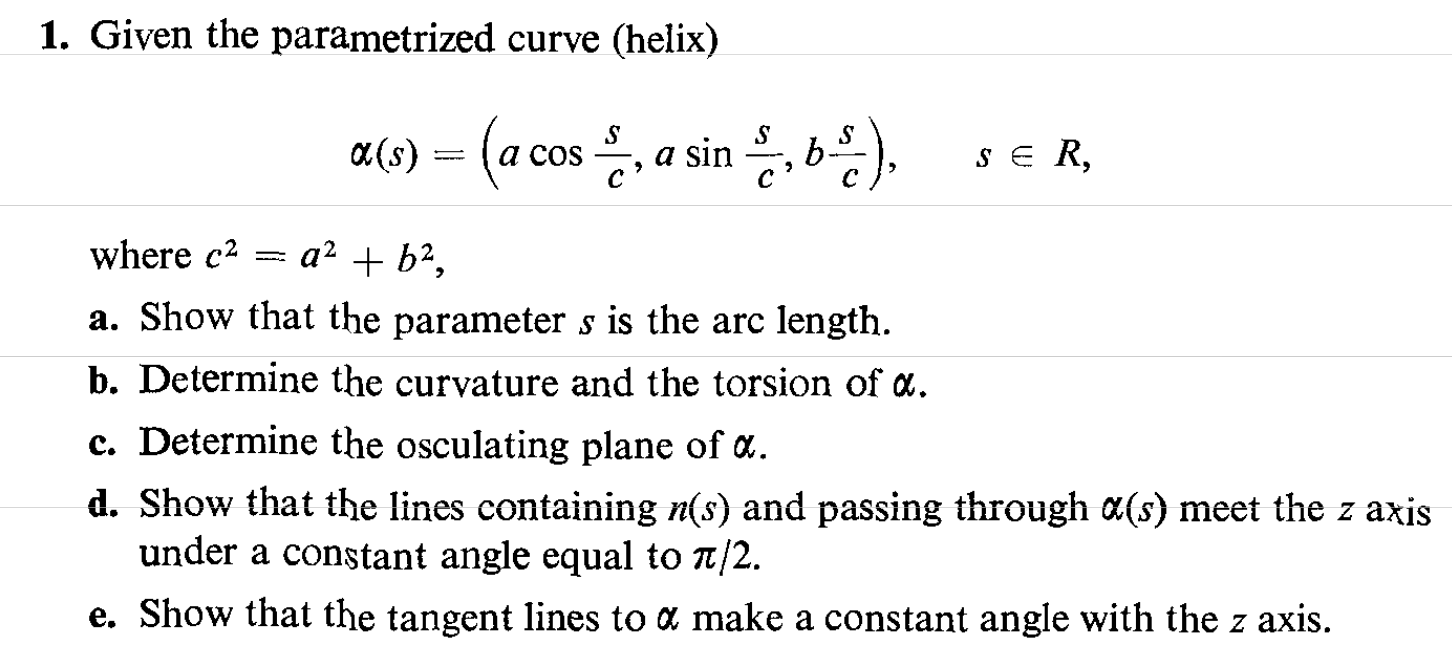
\includegraphics[height=10cm,width=18cm]{hw2q5}
\end{question}
\begin{question}{}{}
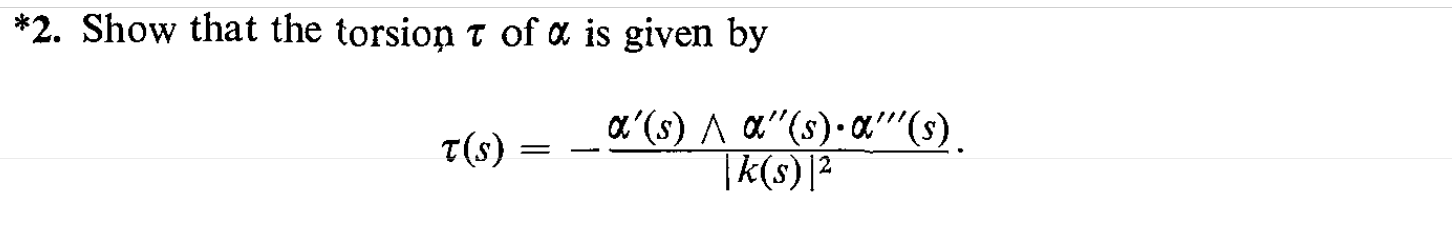
\includegraphics[height=3cm,width=18cm]{hw2q4}
\end{question}
\begin{question}{}{}
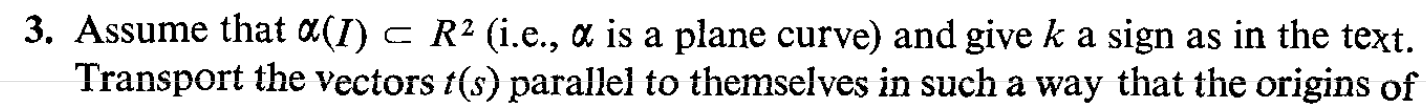
\includegraphics[height=3cm,width=18cm]{hw2q3}
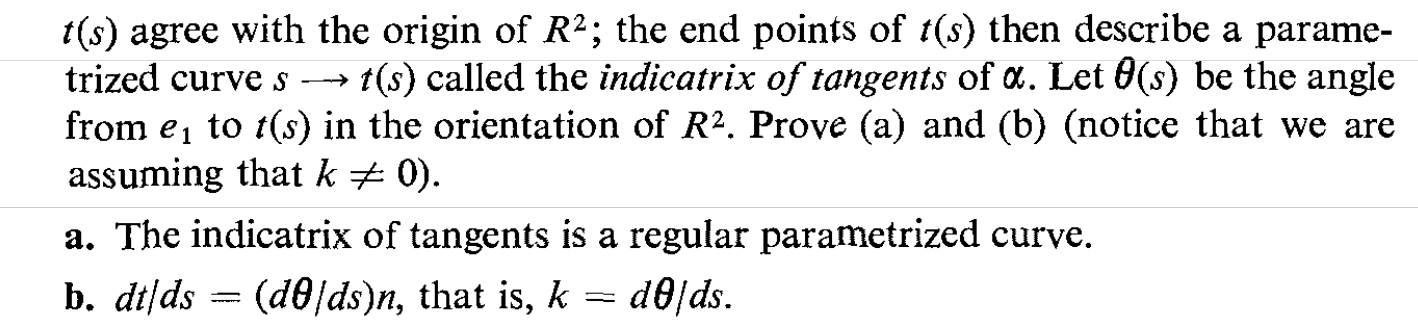
\includegraphics[height=4cm,width=18cm]{hw2q2}
\end{question}
\begin{question}{}{}
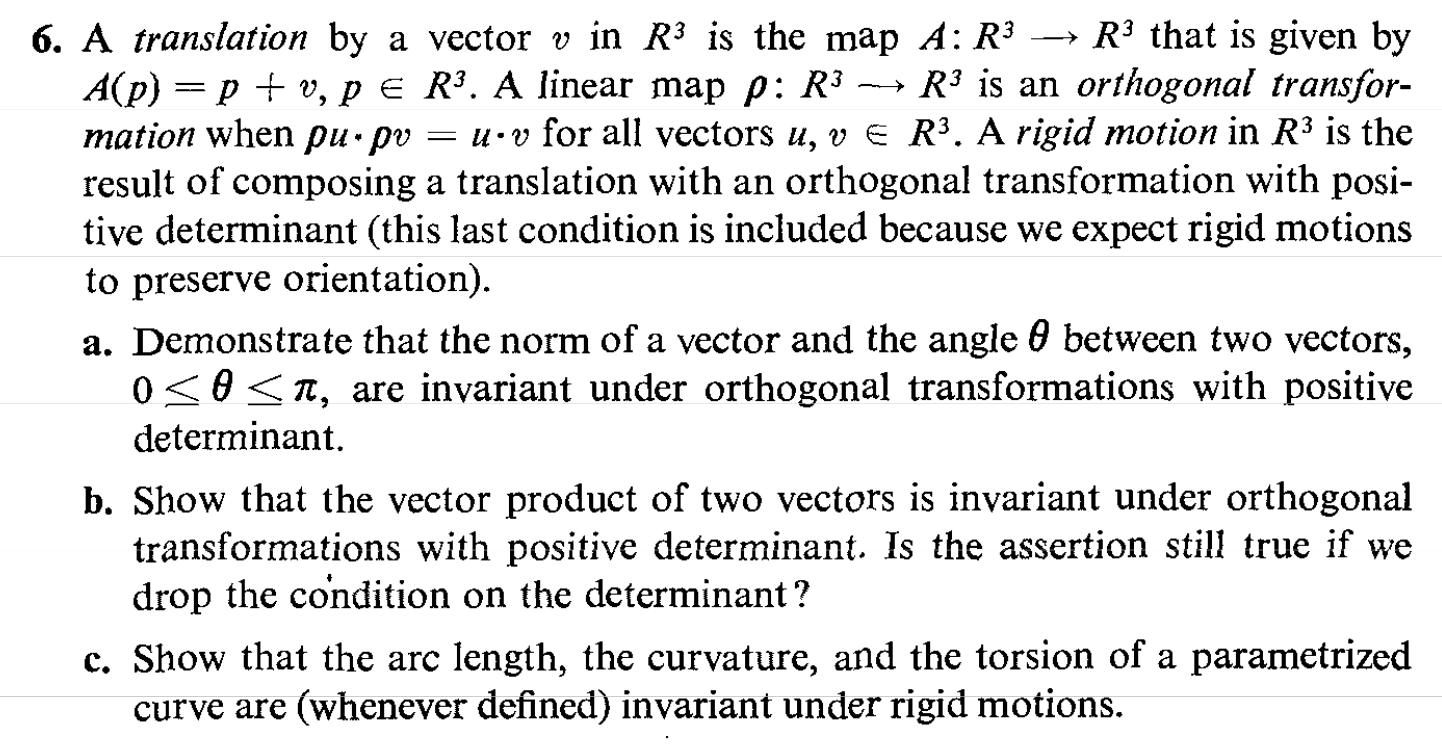
\includegraphics[height=10cm,width=18cm]{hw2q1}
\end{question}

\begin{question}{}{}
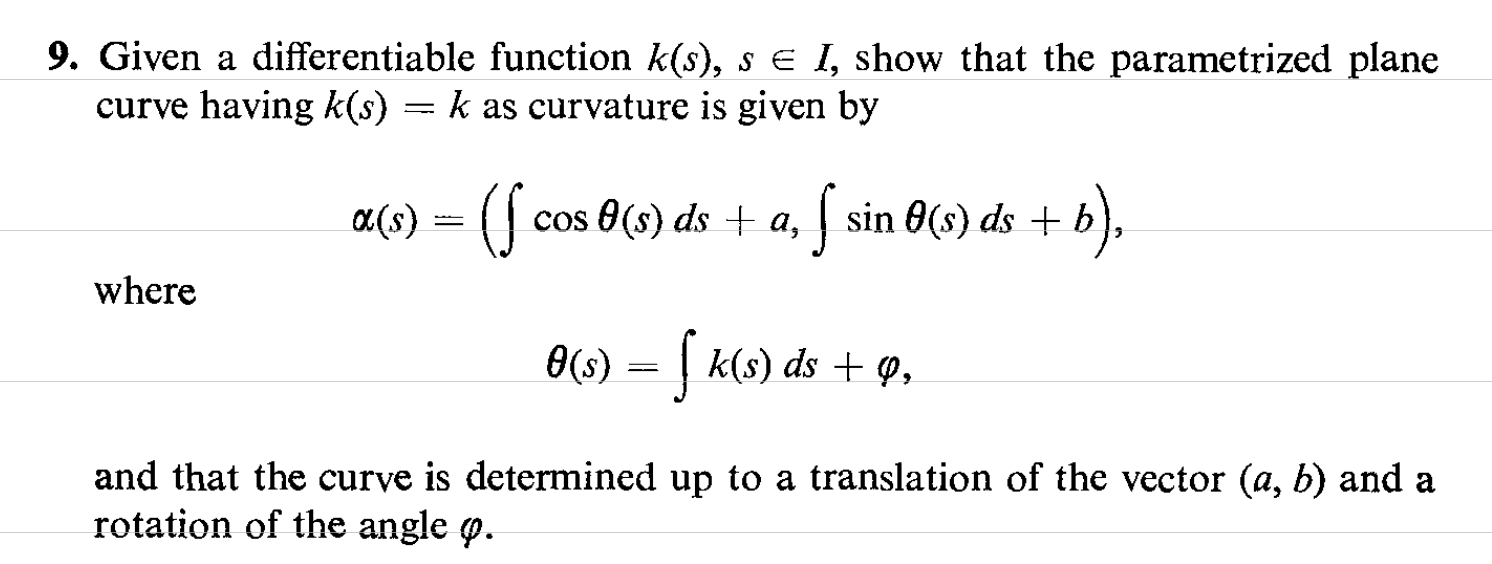
\includegraphics[height=6cm,width=18cm]{hw2q18}
\end{question}
\begin{question}{}{}
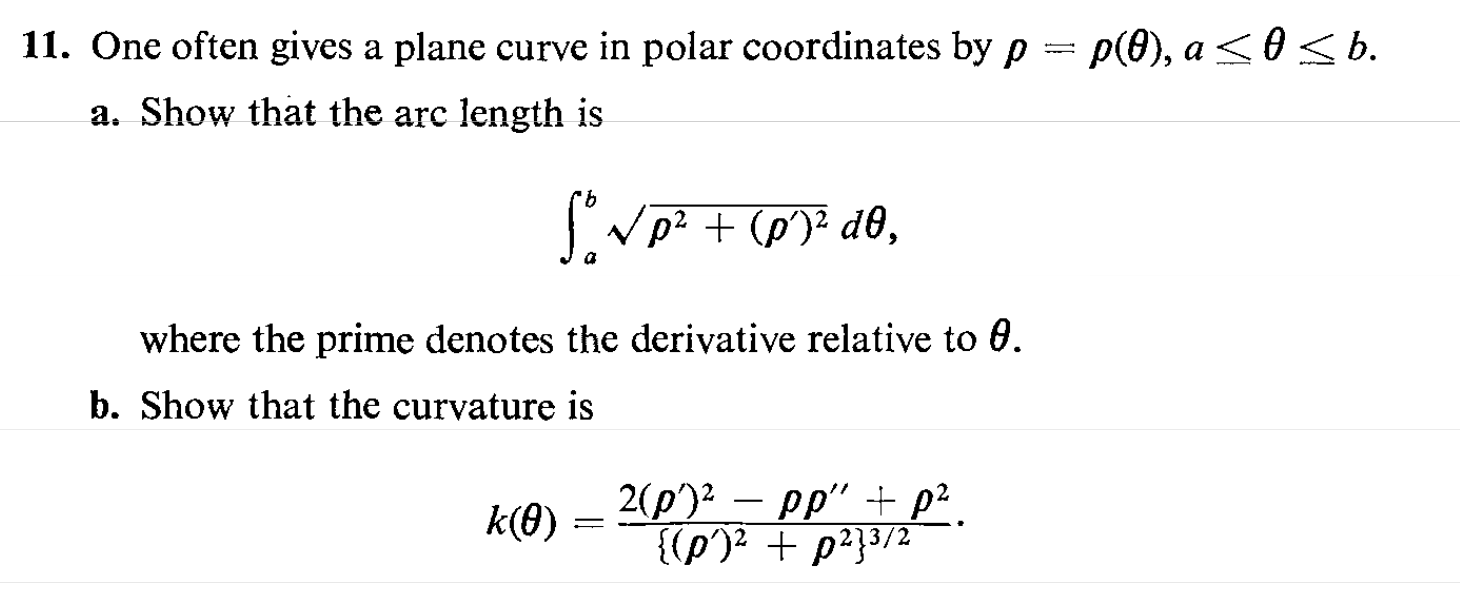
\includegraphics[height=6cm,width=18cm]{hw2q17}
\end{question}

\begin{question}{}{}
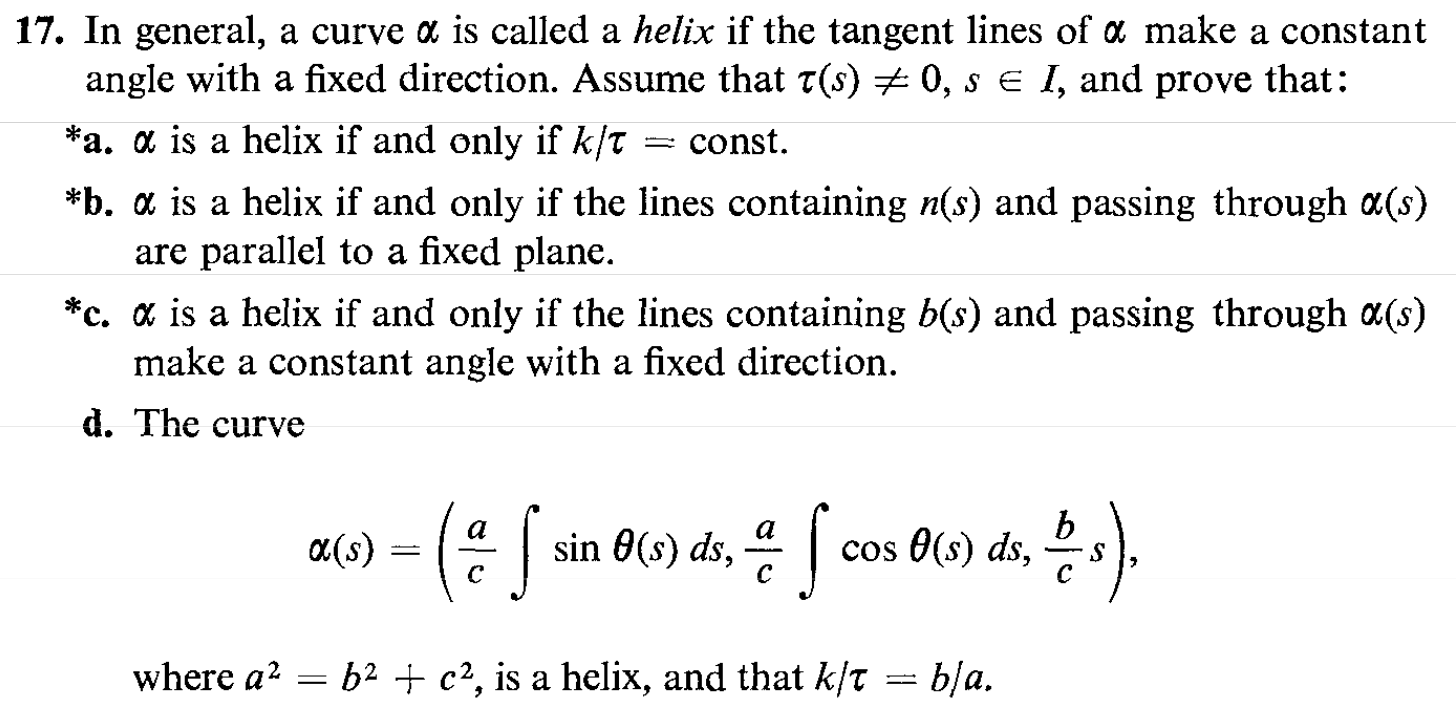
\includegraphics[height=8cm,width=18cm]{hw2q16}
\end{question}
---------------------------------------------------------------------------------------

\begin{question}{}{}
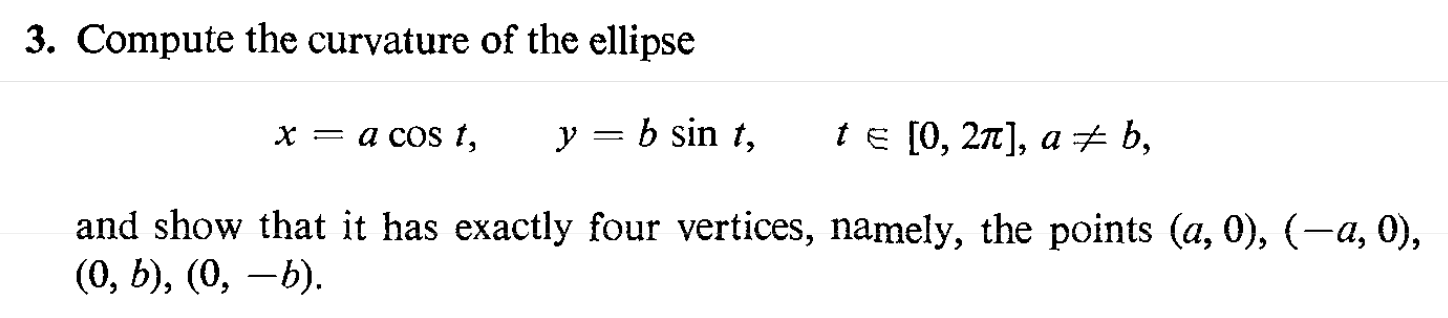
\includegraphics[height=4cm,width=18cm]{hw2q15}
\end{question}


\begin{question}{}{}
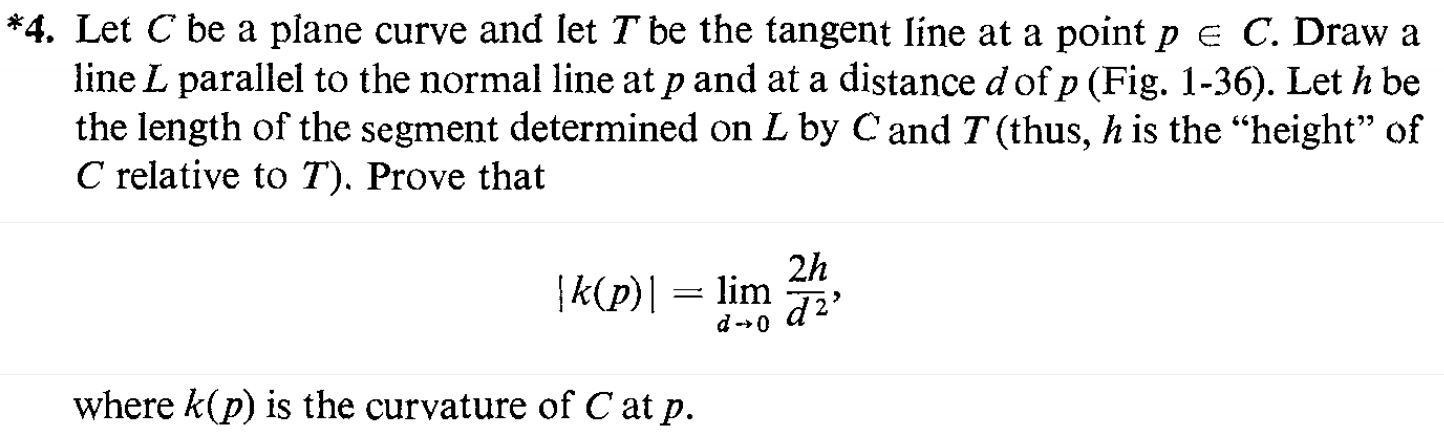
\includegraphics[height=6cm,width=18cm]{hw2q14}
\end{question}

\begin{question}{}{}
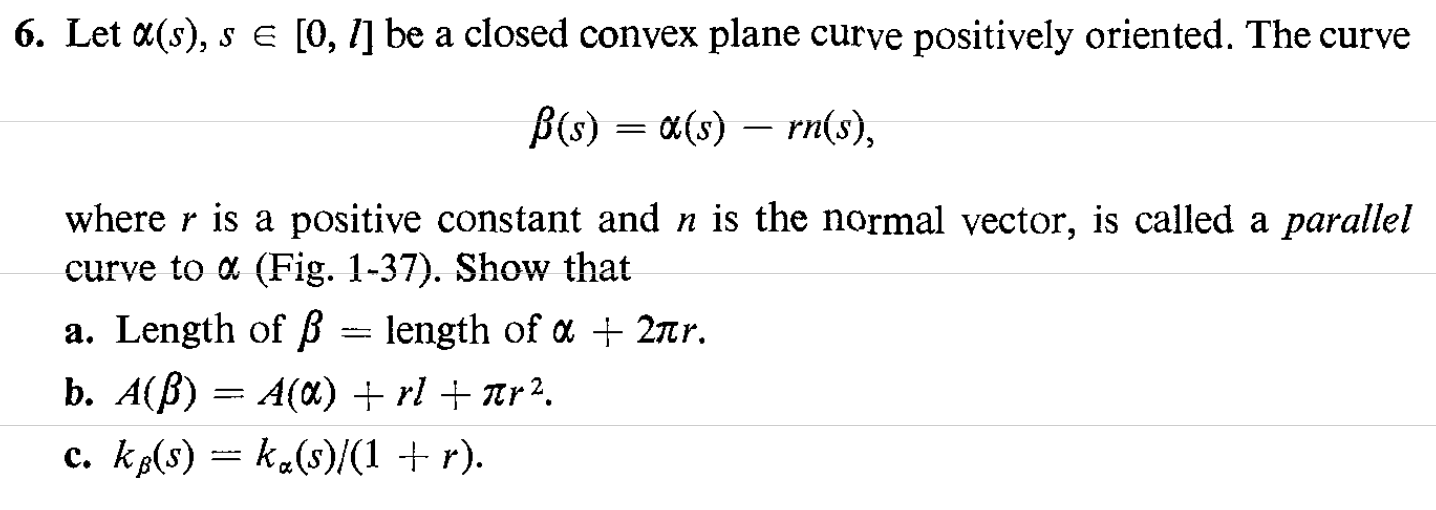
\includegraphics[height=8cm,width=18cm]{hw2q13}
\end{question}


\begin{question}{}{}
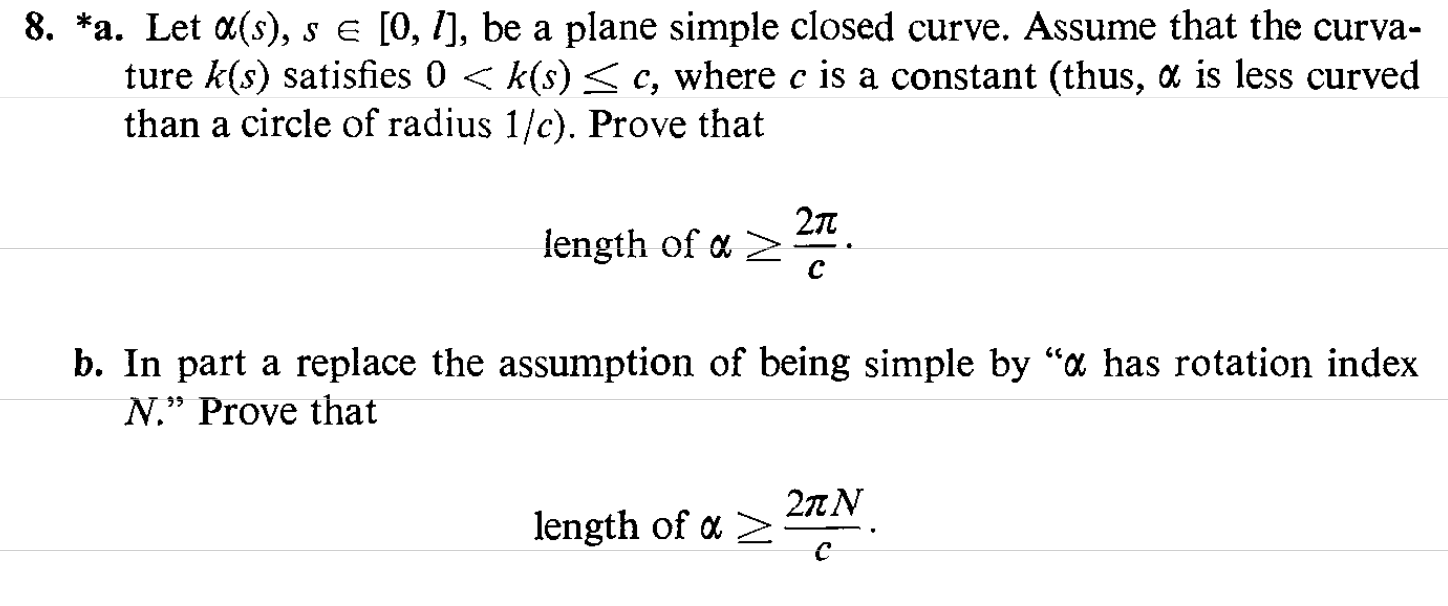
\includegraphics[height=6cm,width=18cm]{hw2q12}
\end{question}
\begin{question}{}{}
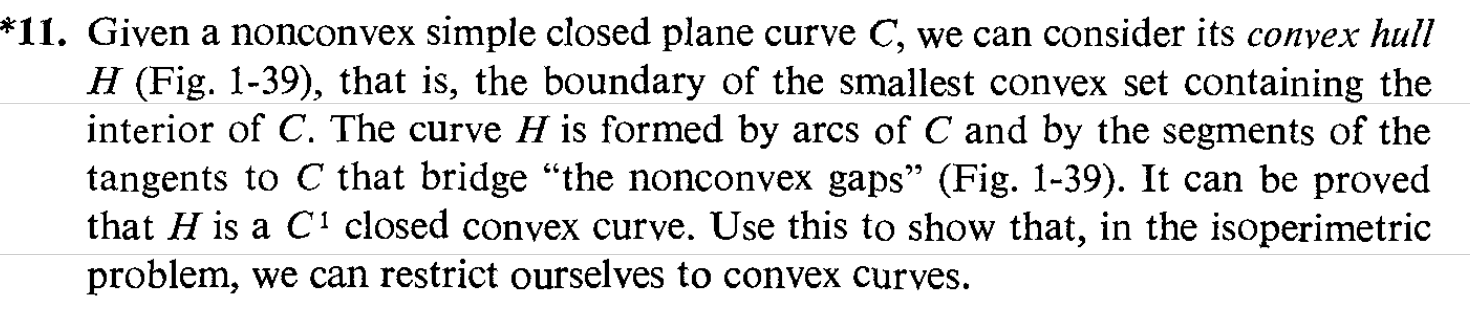
\includegraphics[height=4cm,width=18cm]{hw2q11}

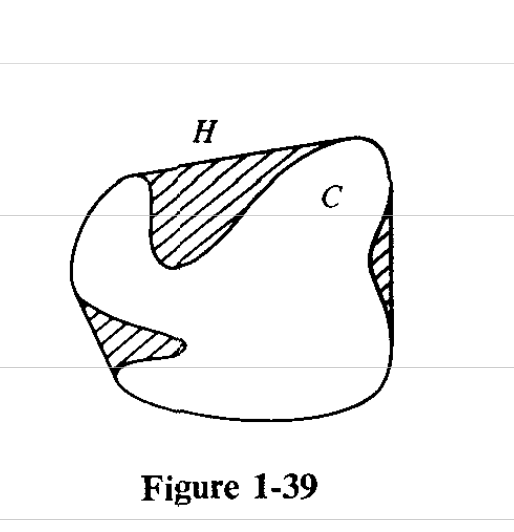
\includegraphics[height=4cm,width=18cm]{hw2q10}
\end{question}
---------------------------------------------------------------------------------------

\begin{question}{}{}
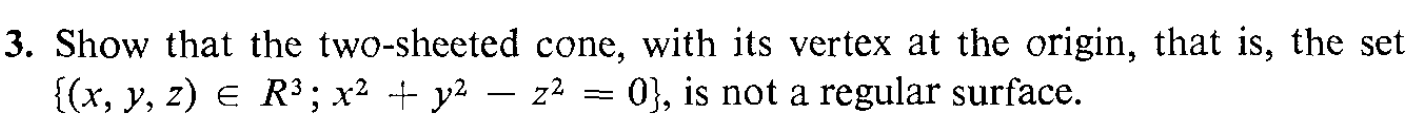
\includegraphics[height=2cm,width=18cm]{hw2q9}
\end{question}
\begin{question}{}{}
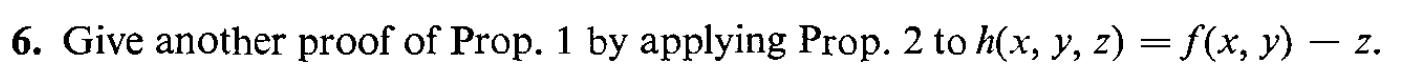
\includegraphics[height=1cm,width=18cm]{hw2q8}
\end{question}
\begin{question}{}{}
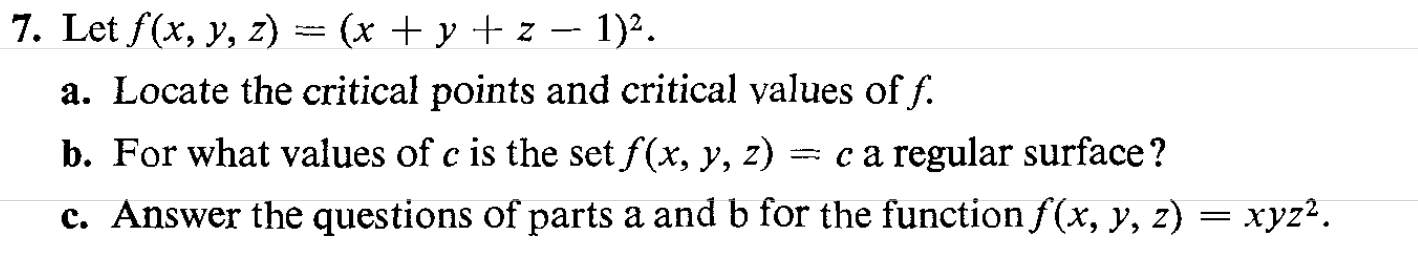
\includegraphics[height=3cm,width=18cm]{hw2q7}
\end{question}

\end{document}
